%\addcontentsline{toc}{chapter}{Development Process}
\chapter{Experiment Methods}
%
%This section should discuss the overall hypothesis being tested and justify the approach selected in the context of the research area.  Describe the experiment design that has been selected and how measurements and comparisons of results are to be made. 
%
%You should concentrate on the more important aspects of the method. Present an overview before going into detail. As well as describing the methods adopted, discuss other approaches that were considered. You might also discuss areas that you had to revise after some investigation. 
%
%You should also identify any support tools that you used. You should discuss your choice of implementation tools or simulation tools. For any code that you have written, you can talk about languages and related tools. For any simulation and analysis tools, identify the tools and how they are used on the project. 
%
%If your project includes some engineering (hardware, software, firmware, or a mixture) to support the experiments, include details in your report about your design and implementation. You should discuss with your supervisor whether it is better to include a different top-level section to describe any engineering work.  

This chapter aims to provide a discussion into the experiments implemented with respect to the investigation detailed in Chapter 1, with emphasis on the adopted approaches adopted and the resulting actions of handling issues encountered.

The results subsequently collected from these experiments are presented in Chapter 3.

\section{Collection of Appropriate Test Data}

Prior to beginning the implementation of any experiments, it was first necessary to identify and collect sets of sample images which would accurately represent the types of input expected upon the deployment of a completed system into a live scenario. 

\subsection{Image Data Requirements}

As discussed previously in Section \ref{assumptions}, for the simplification of the \textit{primary aims} presented in the working hypothesis, the assumption was drawn that at least in early stages of investigation, the system would make exclusive use of images captured from a single camera positioned to face in front of the robot that was also limited to moving in the same direction as the camera (i.e. forward-motion only).

When identifying appropriate test data for use in experiments, a the following characteristics were considered:

\begin{itemize}
	\item The images must provide a reasonable field of view of the current scene above and below the horizon line (i.e it was important to capture objects within the scene located both far away and close to the camera)
	\item The images must show the act of forward translation through the current environment. This would be most obvious through the observation of a vertical displacement in the negative direction (i.e. downwards) visible in features located along the ground plane.
	\item The images must not show forward translation as horizontal movement across the image plane (i.e. no images captured from cameras looking out from the side of a robot moving in a forwards direction).
	\item The images must be of a size and quality reasonably expected of a standard ``point-and-shoot" consumer-grade camera.
	\item The images must have been originally captured in colour, using the ``default" colour space supported by the camera (typically this would be RGB for standard consumer-grade camera).
	 \item The images should demonstrate minimal change in rotation or pitch (i.e. should be taken across a flat surface).
\end{itemize}

In addition to these ``baseline" requirements, additional requirements were also defined with the intention for use within specific experiments focussing on the identification of particular aspects in motion behaviour. These secondary requirements were intended to be used on an ``as needed" basis and came with the possibility of the opposite statement to the ones detailed below being desired in certain situations:

\begin{itemize}
	\item The images should demonstrate minimal rotational motion (i.e. no examples of the robot turning to change direction)
	\item The images should capture terrain that is predominately flat and free of major obstacles both positive (e.g. rocks) and negative (e.g. pits).
\end{itemize}

Unfortunately due to time constraints, some the planned experiments could not be completed within the the major project, as a consequence of this, not all examples of images meeting every one these requirements were captured. However, it was still important to define these requirements before beginning any experimentation and given more time, would still prove to be valid.

\subsection{Existing Datasets}

At the beginning of the project, some time was initially devoted to searching for any existing datasets that could provide suitable imagery. One main advantage to using existing datasets, is that typically other previous projects have already had the opportunity to verify that the data is both accurate, and provides a sufficient level of variability that proves crucial in testing the robustness of the systems that make use them as part of their evaluation.

In the majority of cases, existing datasets also come pre-packaged with appropriately verified ground truth data, thereby preventing the need for projects that subsequently chose to use them having to produce their own ground truth results, consequently saving on both time and resources.

While a number of previously published datasets were found to be available \cite{ucl-dataset}, \cite{baker-dataset}, \cite{mpi-dataset}, unfortunately none were found to be suitable in relation to the requirements detailed in the previous sub-section.   

\subsection{Manual Datasets}

Following the lack of appropriate existing datasets with the field, it was necessary that a bespoke datasets would have to be created manually. While in the short term this meant an increased work load, it also presented the opportunity to capture datasets that would specifically meet the needs of the experiments.

\subsubsection{Camera Rig Setup}

In the pursuit of capturing image datasets, a wide range of approaches could have potentially been adopted. One initial idea considered requesting the use of one of several `Pioneer' robots owned by the Computer Science department at Aberystwyth University. By rigidly mounting a camera to the front of one of these small wheeled robots, and remotely instructing it to move forward by a set distance before manually triggering the camera, it would be achievable to capture a collection of images in which each demonstrated an equal level of displacement between that and the next image. 

As part of a particularly elaborate setup, it would have perhaps been feasible to provide an interface to the mounted camera (perhaps via USB or serial) before programming the Pioneer robot into automatically capturing images at set intervals, while following a pre-determined path through the environment (making use of the on-board sonar and odometry capabilities). 

While these approaches would certainly provide an ample solution, following a discussion with the project supervisor, it was deemed that, at such an early stage in an investigation that was already limited in time remaining, efforts would be better spent focussing on conducting actual research, as opposed to the collection of test data.

Nevertheless, a means of manually capturing image datasets was still required. As such, the decision was taken to adopt a `simplified' approach, that in exchange for greater manual involvement, could consequently be brought into service in a shorter timeframe.

Compared to the use of the robot, this approach was certainly less `sophisticated' in terms of its setup (Figure \ref{fig:rig}), consisting only of:

\begin{itemize}
	\item Two cardboard boxes (one rectangular and one angled);
	\item A consumer-grade ``point-and-shoot" camera (Panasonic Lumix DMC-FS18 (2011));
	\item A standard 30cm ruler;
	\item A standard spirit level;
\end{itemize}

However, as well as being quick to initially build, this setup would go on to prove to be a lot more portable and a great deal cheaper to modify and fix than one of the Pioneer robots. 

\begin{figure}[ht!]
\centering
\includegraphics[scale=0.08]{images/rig_setup}
  \caption{The camera-rig setup used to capture the experiment datasets from the front and back profiles.}
\label{fig:rig}
\end{figure} 

\subsubsection{Capture Locations}

A selection of locations were chosen for the purposes of capturing datasets. To ensure an appropriate level of variability, each dataset focussed on a different type of terrain environment that it was predicted a robot may face during live deployment.

Datasets were captured at four separate locations (Figure \ref{fig:location}), split between indoor and outdoor sites to provide variation in lighting conditions and terrain type:

\begin{enumerate}
	\item \textbf{Site 1:} Living room rug with brightly-coloured simple-shapes (Indoors) (Natural light entering from the right)
	\item \textbf{Site 2:} Brick-paved road (Outside) (Natural light)
	\item \textbf{Site 3:} Heavily-patterned asian rug upon white-tiled floor (Inside) (Partial natural light from behind camera, partial artificial light)
	\item \textbf{Site 4:} Slate-tiled footpath (Outside) (Natural light)
\end{enumerate}

\begin{figure}[ht!]
\centering
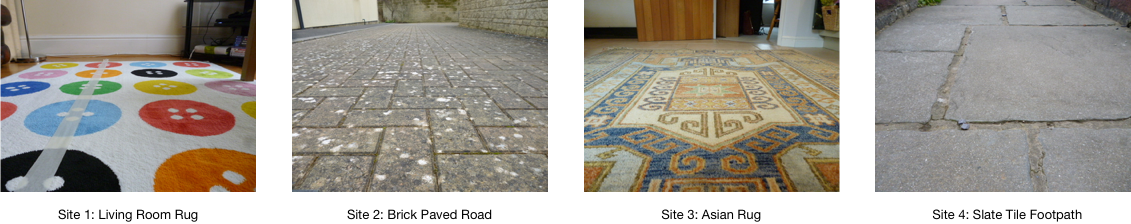
\includegraphics[scale=0.35]{images/locations.png}
  \caption{Examples of the first frame captured from each of the four location datasets.}
\label{fig:location}
\end{figure}

\clearpage
\subsubsection{Capturing Process}

The method behind the use of the `homemade' camera rig to capture the image datasets also proved simple in design. This was regarded as favourable, given that it relied on manual involvement where human error subsequently becomes a potentially big issue. 

Figure \ref{fig:flow} below details the outline of the method used to capture an individual image dataset.

\begin{figure}[ht!]
\centering
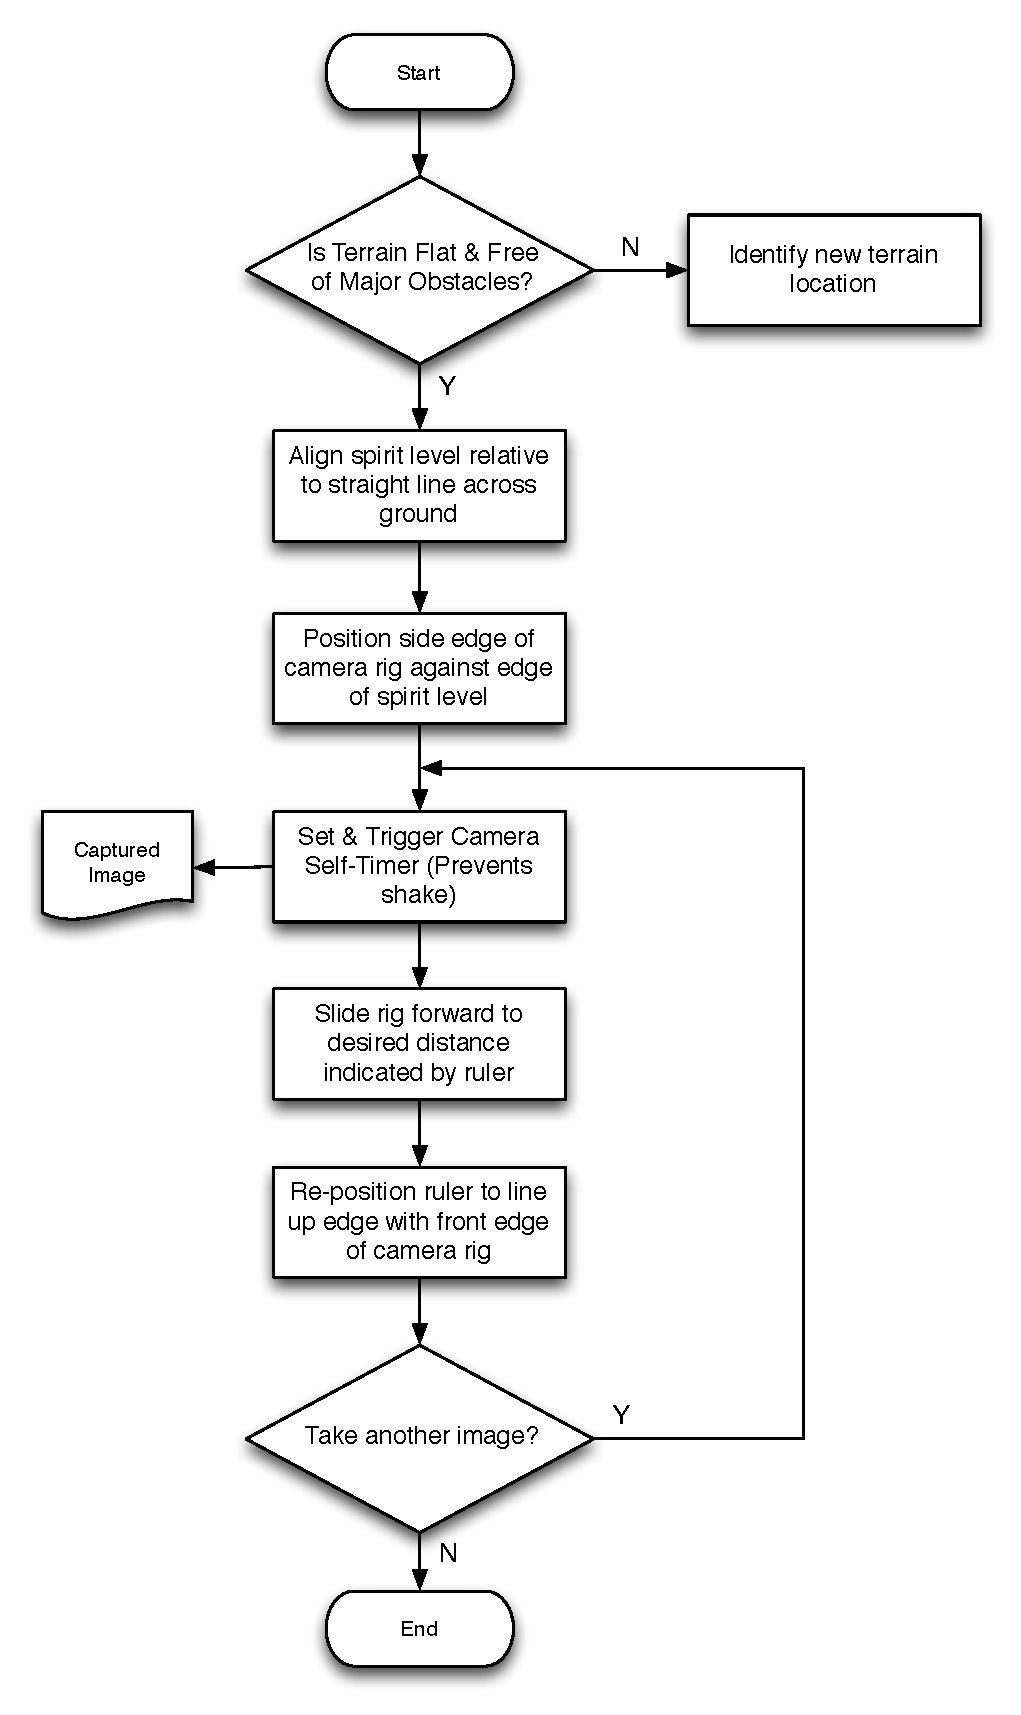
\includegraphics[scale=0.6]{images/camera_flow.pdf}
  \caption{General method process employed for capturing dataset images.}
\label{fig:flow}
\end{figure}

While the method for capturing images followed a ``fixed" procedure, it did allow for changes in the type of terrain captured, and the level of set displacement by which the camera was moved between subsequent images.



\subsubsection{Calibration of Physical Setup}

Although one of the aims of the hypothesis was to avoid the need for calibration of the camera, it was decided that in the interests of good experiment practice, measurements regarding the physical setup of the camera rig should be taken. 

\begin{wrapfigure}{r}{0.5\textwidth}
\vspace{-20pt}
  \begin{center}
    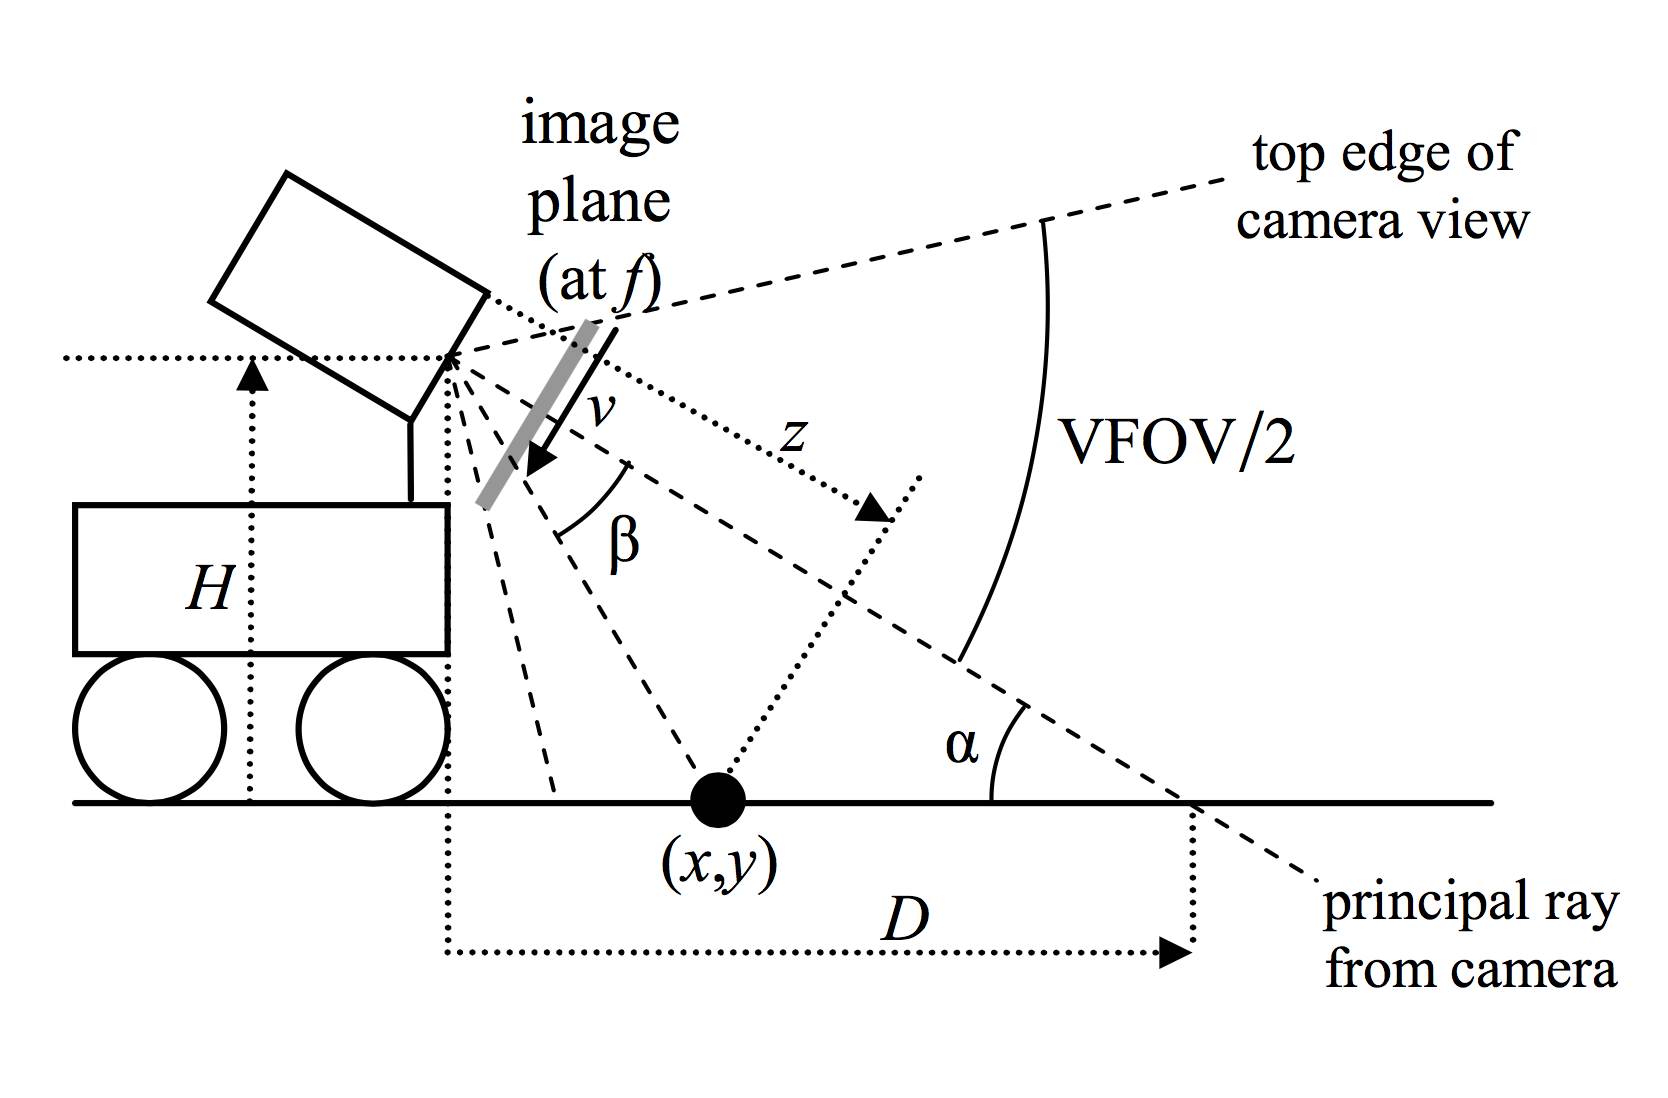
\includegraphics[width=0.49\textwidth]{images/cam_setup.png}
  \end{center}
  \vspace{-10pt}
  \caption{Diagram originally produced by Campbell \textit{et al.} \cite{campbell} depicting the physical setup of the camera rig used within their work. The camera rig built for this project followed a very similar setup.}
  \label{fig:setup}
  \vspace{2pt}
\end{wrapfigure}

Following the process outlined in the work of Campbell \textit{et al.} \cite{campbell}, the calibration would provide a future opportunity, should the need arise, to calculate the mapping between coordinates in the image plane and the ground plane.

The physical setup of the camera rig matched the same general setup as described by Campbell \textit{et al.} \cite{campbell} (Figure \ref{fig:setup}), where $h$ refers to the height of the camera from the ground, and $d$ refers to the distance between the front edge of the rig base and the position at which the principle ray from the camera lens intersects with the ground plane \cite{campbell}.

To establish the distance $d$, a target $T$ was positioned on the ground such that it lay within the centre of the camera's viewfinder (Figure \ref{fig:target}). The distance between the position of the target $T$ and the front of the rig was then manually measured in order to arrive at the final length. 

After also manually measuring the height $h$, it became possible to calculate the tilt $ \alpha $ of the camera using basic trigonometry:

\begin{equation}
	\tan(\alpha) = \frac{h}{d}
\end{equation}

%\textbf{Note to the reader:}
%
%The remaining steps of the calibration model outlined below did not form part of the main project investigation, however following the decision by the author to investigate them as part of improving their own understanding, they have been included in this report for completeness.
%
%
%The next step was to define the relationship between the vertical offset of a point in the image $v$ and the associated vertical angle between that same point and the principle point along the ground plane $\beta$ \cite{campbell}:
%
%\begin{equation}
%	\tan(\beta) = (2v - V)\tan(\frac{VFOV}{2})
%\end{equation}  
%
%where $ V $ refers to the height of the image in pixels, and $VFOV$ represents the vertical field of view from the camera:
%
%\begin{equation}
%	VFOV = 2\tan^{-1}(\frac{d}{2f})
%\end{equation}
%
%where (in this case) $d$ represents the vertical dimension of the camera sensor (but can also represent the horizontal dimension if wishing to calculate the horizontal FOV), and $f$ represents the camera focal length \cite{bourke}.
%
%Obtaining values for $d$ and $f$ involved consulting the manufacturer specifications document for the camera \cite{camera-spec}, in which the following information was identified:
%
%\begin{itemize}
%	\item \textbf{Sensor Type:} 1/2.33" CCD
%	\item \textbf{Lens Aspect Ratio:} 4:3
%	\item \textbf{Focal Length:} 5-20mm 
%\end{itemize}
%
%In calculating $d$, there was some confusion about how to establish the dimensions of the sensor from the published sensor type. It was assumed initially that the diagonal dimension of the camera would match that of dimension representing the sensor type (i.e. 1/2.33"). 
%
%However following some further research, it came to light that this was not the case, and in fact the dimension listed as the sensor type was not representative of the true sensor size, but instead was one of many industry-standard type designations used to classify image sensors \cite{gum}. Subsequently, the vertical dimension of the camera sensor was obtained using an online guide providing dimensions for standard types of sensor \cite{bockaert}.
%
%The final step in the calibration process published by Campbell \textit{et al.} \cite{campbell} involved recovering the distance $y$ from the observed point along the ground plane to the camera rig:
%
%\begin{equation}
%	y = \frac{h}{\tan{\alpha + \beta}}
%\end{equation}
%
%and the associated depth $z$:
%
%\begin{equation}
%	z = \frac{H\cos(\beta)}{\sin(\alpha + \beta)} 
%\end{equation}
%
%Through the use of this calibration model, the actual displacement of any point along the ground plane that is represented in the image plane, can be calculated by taking into account the depth between that point along the ground plane and the camera \cite{campbell}.


\subsection{Artificial Datasets}

While unfortunately never pursued in this project due to time limitations, an alternative approach to gathering robust testing data was to capture motion sequences set within a 3D virtual environment. 

A key advantage of creating artificial image datasets stems from the level of control that becomes available over properties including the choice of lighting, terrain textures and landscape geometry. This high degree of granularity that makes using computer-generated datasets a popular choice for many vision-based projects, perhaps especially within earlier stages of a project, where one is simply attempting to identify bugs in the system, rather than evaluating hypotheses \cite{ucl-dataset}, \cite{baker-dataset}, \cite{mpi-dataset}.
 
Other potentially very useful consequences of using computer-generated datasets include control over the amount of noise an image may contain (e.g. choice to include or remove specular reflections), and the high degree of speed at which new datasets adopting different condition configurations could be created almost ``on the fly" in order to test new ideas and approaches within an experiment. 

\begin{wrapfigure}{l}{0.5\textwidth}
  \begin{center}
    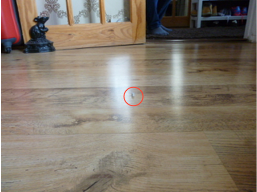
\includegraphics[width=0.45\textwidth]{images/cam_target.png}
  \end{center}
  \vspace{-10pt}
  \caption{Image indication the visual target used as part of the manual calibration of the camera rig setup.}
  \label{fig:target}
  \vspace{-20pt}
\end{wrapfigure}

The creation of artificial datasets would have provided an opportunity to test the robustness of the experiment methods against a much broader range of conditions than what was feasibly possible using only real-world imagery. However the use of datasets captured from real-world environments was still arguably the most crucial in terms of evaluating the performance of experiment methods, given that these would ultimately provide the closest representation to the input expected within a live deployment. 
%
%While there was no time available for the author to learn how to build 3D environments for use in artificial datasets, some simple 2D-shape image datasets were created as part of evaluating the correct functioning of the template-matching approach adopting geometric scaling (discussed further in Section \ref{tm-scaled}).

\section{Establishment of Ground Truth}

With respect to scientific investigation, the term ``\textit{ground truth}" refers to measurement data or results that are known to represent the \textit{absolute truth} of a particular condition or observation which subsequently can be used to determine the accuracy of reported results from a system or method currently undergoing testing and evaluation.

In the context of computer vision, ground truth data will represent observations within image datasets that are known to exist in the real-world, and be accurate.

Due to the very nature of what ground truth data represents, generating such data can still typically only be accomplished through means of manual verification, where human observation continues to be deemed as the `state of art' in terms of providing the best possible accuracy available as to the \textit{fundamental} truth of a condition or observation \cite{kondermann}. 

A fundamental issue with this approach to the collection and verification of ground truth data, is it tends to be costly in terms of both time and resources. Kondermann \cite{kondermann} states that this large requirement in effort to generate ground truth data in combination with its relatively limited applicability in terms of evaluation, consequently results in many vision-based projects failing to provide reference data that is either comprehensive or accurate.

For particular types of reference data, some semi-automated methods do exist for gathering high-accuracy measurement results (e.g. extracting depth information about a 3D environment using laser scanning techniques) \cite{haltakov}. However, these approaches still require at least some manual verification in ensuring that this accuracy is at a level sufficient enough for it to be trusted as ground truth.

In terms of generating ground truth, one of the most challenging types of visual behaviour to document is optical flow \cite{kondermann}. This is because no sensor currently exists that is capable of detecting the effects of optical flow directly, and in most situations (except perhaps within very simple artificial datasets) attempting to perform manual annotation also proves to be an extremely difficult task to achieve with the kind of accuracy that is expected for use as ground truth data \cite{haltakov}. 

%As this was a problem that had potential implications for this project, thoughts began to turn to ways of developing a utility application that could assist a human in manually generating ground truth data for the observed displacement of features across a series of images. 

%\subsection{Ground Truth Utility Tool}
%
%Following discussions with the project supervisor a simple, yet effective solution was devised for determining the vertical displacement between a series of images. 
%
%For each image dataset, it was proposed that an additional pair of images would also be captured for the exclusive purpose of establishing ground truth. While obtained using the exact same method as the rest of the dataset, these two images would differ from the main collection by the addition of a ruler positioned within the centre of each image. The choice to capture the ruler would be important, as the measurement increments it possessed would allow a user to clearly identify the same `feature' within both images (e.g. find the 10cm mark in both images).
%
%The next stage involved the design and implementation of a, GUI-based utility tool that would allow a user to perform the following actions:
%
%\begin{enumerate}
%	\item Load in the pair of dedicated ground truth source images;
%	\item Using the mouse, click to select a number of `feature points' that the user deemed easily-identifiable within the first image (e.g. a particular measure mark along the length of the ruler);
%	\item Cycle through each `feature point' identified in the first image, and click on the location corresponding to the new position of that same `feature point' within the second image;
%	\item Export the calculated ground truth measurements for use in future experiments. 
%\end{enumerate}
%
%Following this process, a collection of sparse measurements would be obtained detailing the calculated number of pixels between the Y-coordinate of a `feature point' located in the first image, and the Y-coordinate of the corresponding `feature point' subsequently located within the second image. As it would not be possible for a user to manually identify and select features at an individual pixel level, interpolation would be required to estimate the intermediate values in order to arrive at a recorded displacement for every row in the image.
%
%Naturally, as with any means of human verification this approach was susceptible to human error in terms how accurately a user could position their mouse upon a feature, and also ensuring that they matched the correct features to each other. However, following the conclusions of a number papers within this topic area \cite{kondermann} \cite{haltakov}, human verification was deemed to still provide the best possible level of accuracy for generating ground truth data relating to optical flow.

\textbf{Note to the reader:}

Within the context of the experiments that were conducted it was agreed by both the author and the project supervisor that in the interests of time, the expected behaviour predicted in the hypothesis (namely  ``\textit{greater vertical displacement is shown approaching the bottom of an image than towards the top}") would serve as sufficient `un-official' ground truth from which the performance of the methods implemented could be evaluated.

\section{Design of Experiment Setup}

Prior to beginning the implementation of specific experiments, it was first necessary to design and implement an underlying software infrastructure with the aim of maximising the \textit{efficiency}, \textit{flexibility} and \textit{repeatability} of the experiments conducted:

\begin{itemize}
	\item \textbf{Efficiency:} The testing infrastructure should execute each experiment in a way that makes efficient use of data and system resources (including but not limited to: imagery datasets, experiment parameters and host computer CPU and memory allowance).
	\item \textbf{Flexibility:} The testing infrastructure should provide support for conducting an experiment under multiple combinations of method parameters entered by the user prior to initiation.  
	\item \textbf{Repeatability:} The testing infrastructure should ensure that each run of an experiment is treated as new and conducted in complete isolation to any previous run. 
\end{itemize}

\subsection{Programming Languages}
\label{lang}

For this project, it was primarily the selection of specific external libraries that determined the programming languages that would be adopted.

The original intention saw the entire project developed in C++, as this matched the `native' development language of the OpenCV library \cite{opencv} that was expected to provide a significant contribution to the implementation of the appearance-based similarity measures under investigation. While the OpenCV library did provide a comprehensive range of bindings for other programming languages including Python, Java and C\#, it was felt that choosing to develop in C++ would prove to be the most beneficial in terms of maximising available functionality (i.e. not all functions within OpenCV were available for alternative languages) and maximising the level of support available from both official documentation and the wider community. 

Following the completed implementation of the \textit{first experiment} (detailed in Section \ref{ex1}), this original intention was altered to instead change from C++11 to Python 2.7 as the primary development language. 

This decision was not taken lightly, with the author being very much aware that by choosing a language with which they were unfamiliar, there was a high probability of the project incurring delays resulting from both learning the actual language, while also having to most likely dedicate additional time to fixing ``common" bugs typically associated with being new to the language. In spite of this, it was decided that while it may potentially cost time in the short term, switching to Python would provide a number of key benefits in the long term. 

The first of these benefits was that in comparison to C++, the language provided significantly more functionality ``out of the box" due to it being situated at a ``higher" level programmatically. While reviewing the implementation of the first experiment, it was found that on a number of occasions, a function that had to written manually in C++ (e.g. standard deviation and variance of a numeric collection), was already available within either the Python language as standard, or one of its primary third-party libraries (e.g. \textit{Numpy} \cite{numpy}). While it was true that many of these functions did not take particularly long to implement in C++, there was a clear benefit to having such functions already implemented in libraries that were known to be both optimised and peer-tested. 

Secondly, following research into the Python language, it soon became clear that it was a popular choice amongst scientific and engineering teams due mainly to its impressive level of support for scientific and numeric computing \cite{perez} and promotion of `natural language' within its syntax that is known to aid in supporting rapid prototyping \cite{ramanujam}. These were both characteristics that could be applied to the needs of this project, and hence were deemed beneficial to future development.

%Thirdly, the process and technologies used to deploy Python applications appeared to be significantly less complicated than that for C++ applications. While  

A further reason for switching to the Python language, which would in time become one of the most significant, was the prospect of being able to make use of the \textit{iPython} interactive computing library \cite{ipython}. Following the discovery of this library during research looking into the use of Python within scientific applications, it became apparent that it had the potential to provide significant capabilities in terms of supporting the automated execution and presentation of experiments and their results. This approach provided a more  intuitive means of displaying and analysis than what was originally available using just a command-line based interface. 

One of the most commonly noted disadvantages of using Python describes the fact that as a scripted language, its general performance is considered to be slower overall than that of compiled languages such as C++. While this was initially of some concern, it was later addressed through the use of a third-party library (Cython \cite{cython}) that enabled computationally expensive functions originally written in Python to be converted automatically into compiled C code.

\subsection{Development Tools}
\label{develtools}

Given the author's lack of prior knowledge in C++ or Python, it was decided that the use of an IDE for development would be most suitable for development, as they would be able to provide support facilities including code completion, automatic refactoring and powerful debugging facilities. 

For C++ development, the Xcode IDE\footnote{\url{https://developer.apple.com/xcode/}} was chosen. While this was primarily a decision based on ease of having the IDE already installed, Xcode did provide a high level of support for managing the deployment of C++ applications, including a facility to automatically generate the `Makefiles' used to install the released version on another computer. 

\begin{wrapfigure}{l}{0.6\textwidth}
	\vspace{-10pt}
  \begin{center}
    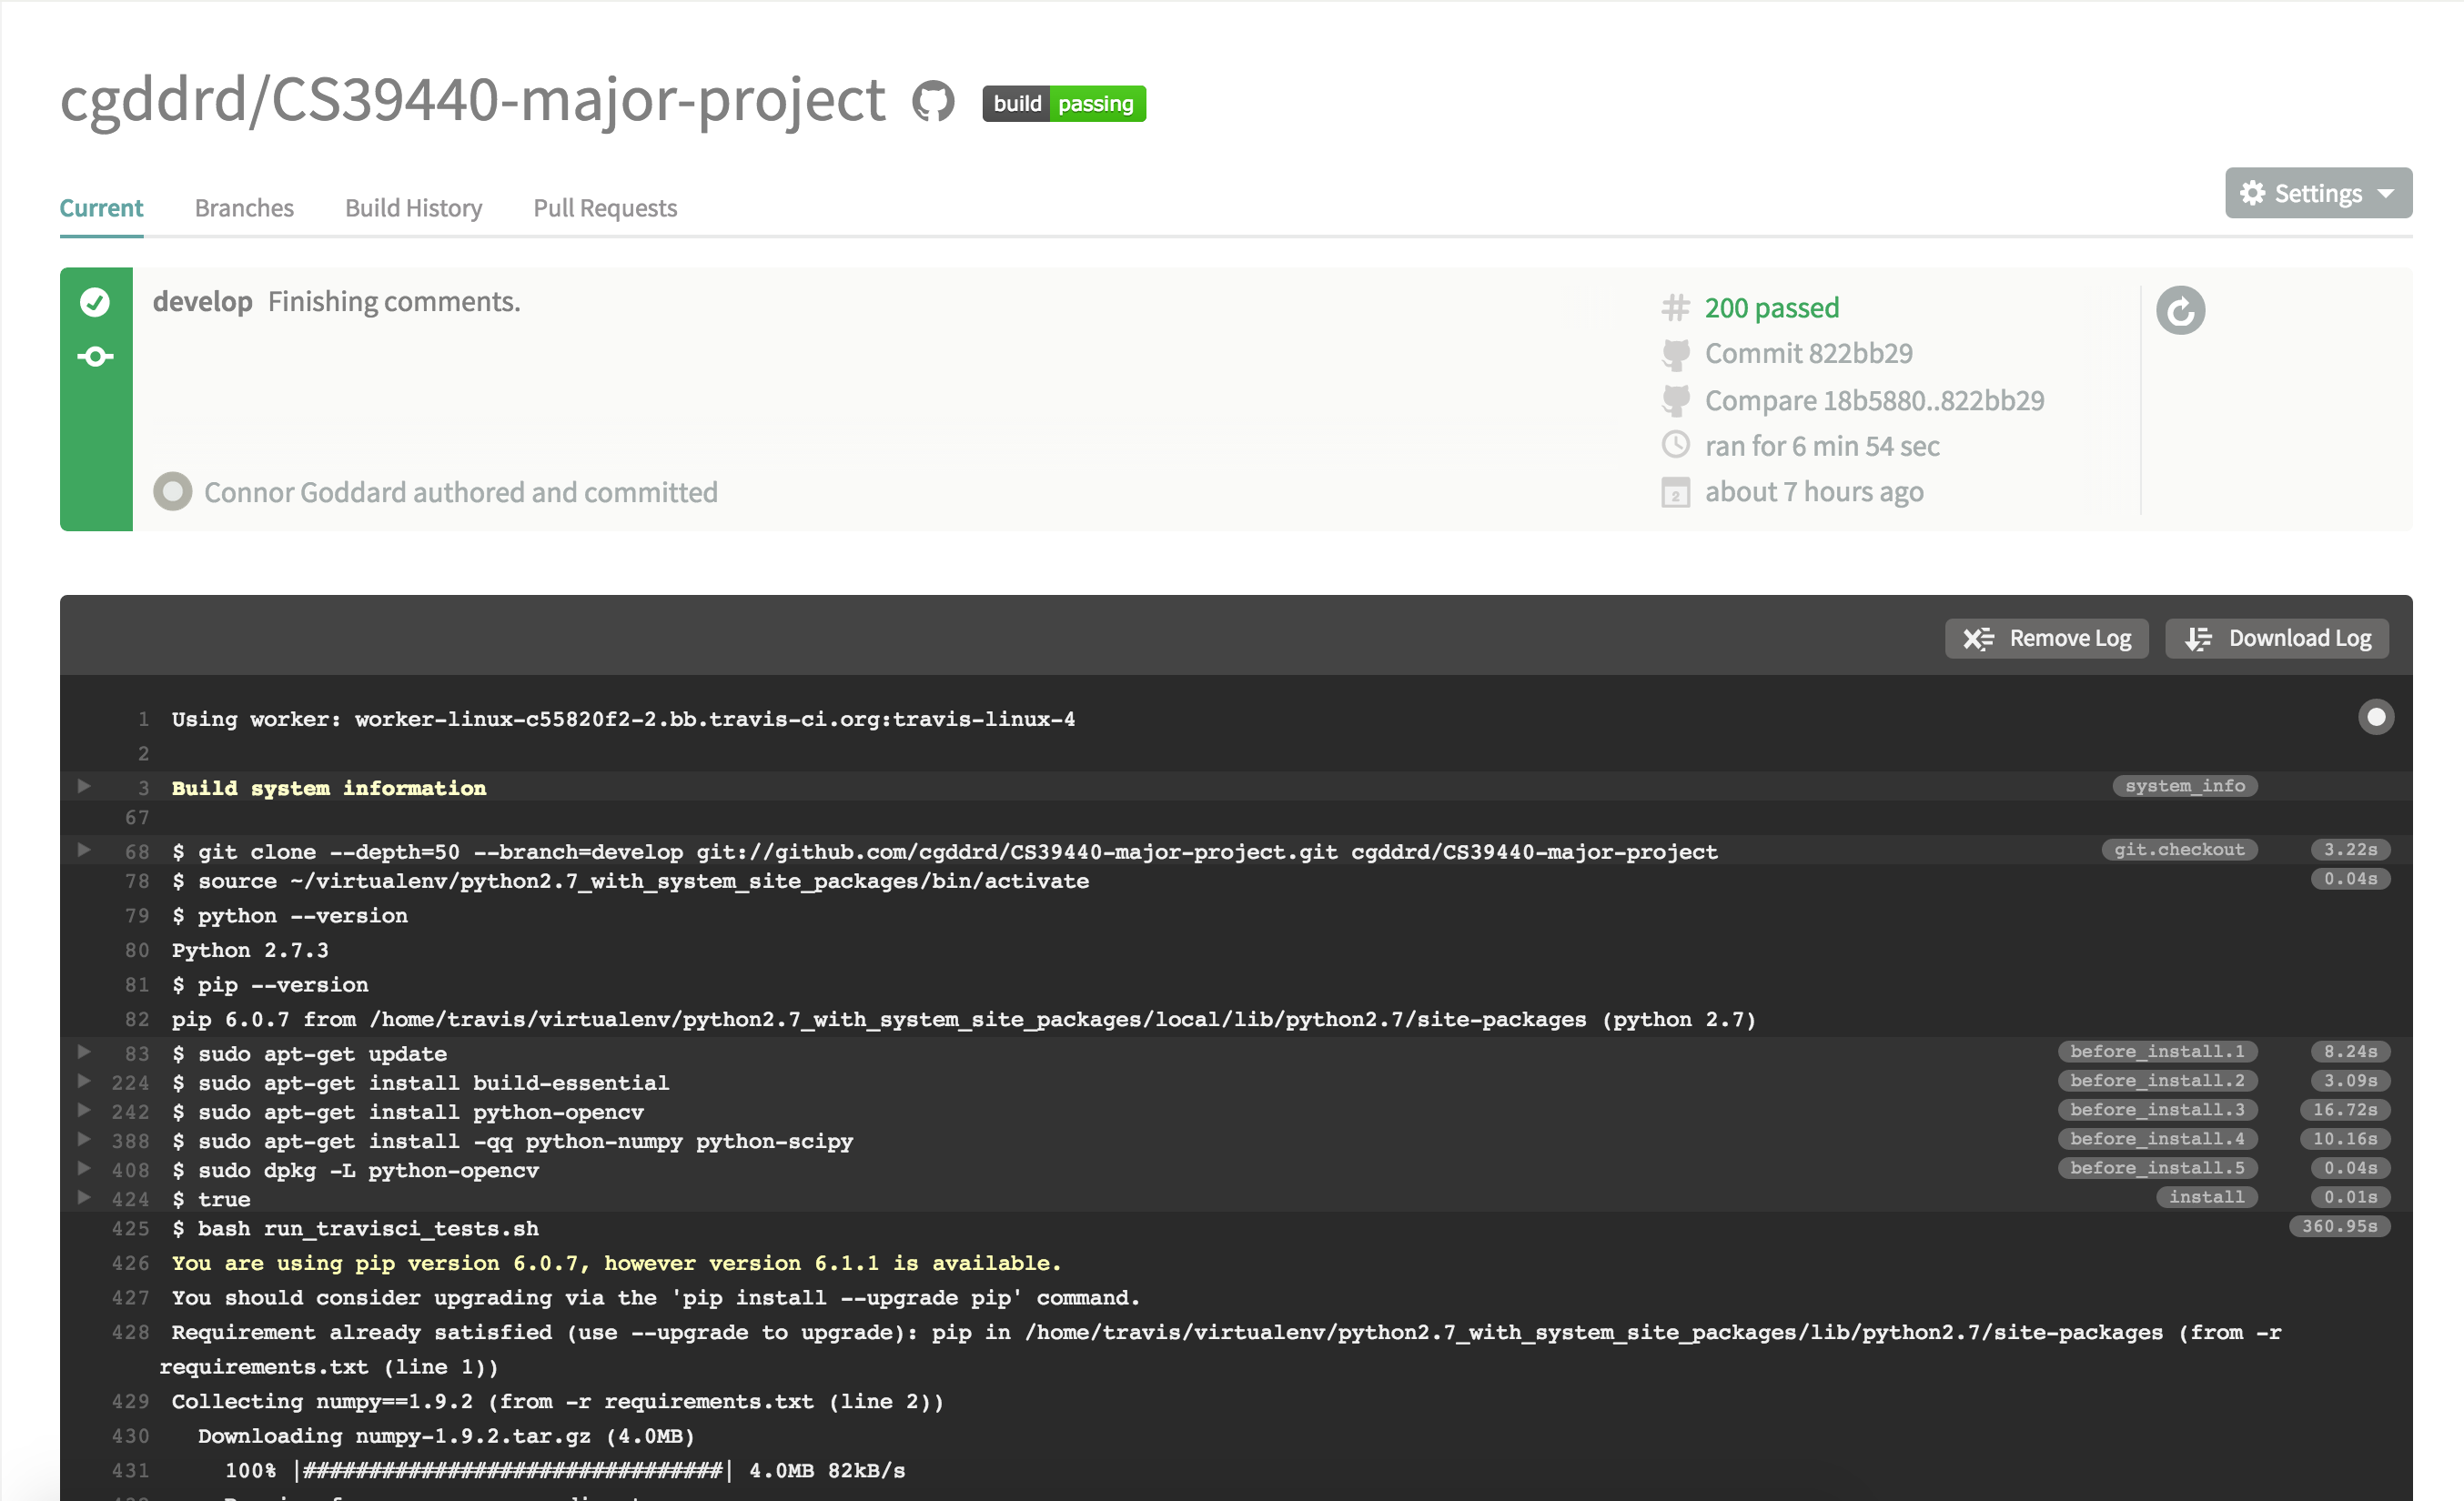
\includegraphics[width=0.55\textwidth]{images/travisci.png}
  \end{center}
  \vspace{-10pt}
  \caption{Travis CI provided automated builds and test suite execution upon each commit to the Github repository}
  \label{fig:target}
  \vspace{-10pt}
\end{wrapfigure}

Python development was conducted within the PyCharm IDE\footnote{\url{https://www.jetbrains.com/pycharm}} making use of the educational license provided by JetBrains. Of particular benefit was the support provided for the automatic management of external dependencies and libraries, which included the ability to export a complete list of a project's dependencies and their precise version numbers.

Version control was managed by git, with repositories hosted on both Github\footnote{\url{https://github.com/cgddrd/CS39440-major-project}} and a separate private git server. The project also made use of the Travis CI\footnote{\url{https://travis-ci.org/cgddrd/CS39440-major-project}} continuous integration platform to provide automated building and testing of software. Integrating directly with the Github service, new builds would be triggered automatically upon pushing of a new commit to the remote repository. Should any part of the build process fail (including unit test failures), the service would send an email notification detailing the type and source of the error.  

\subsection{Core Libraries}
\label{libs}

The project made use of a selection of libraries to support in the development of the both the experiment testing framework, and the experiment methods themselves. 

The \textit{OpenCV} library \cite{opencv} became a vital tool in the development of this project, providing a large number of ``core" image processing and computer vision facilities including colour space manipulation, sub-region extraction and template matching (see Section \ref{templmatchopencv}). This project referenced the latest stable release at the time of writing (2.11.0), and made use of both the C++ and Python bindings as discussed in Section \ref{develtools}.

For aspects of the implementation developed in Python (approximately 75\% of code written), the project made extensive use of the \textit{Numpy} \cite{numpy}, \textit{Cython} \cite{cython}, \textit{Matplotlib} \cite{matplotlib} and \textit{iPython} \cite{ipython} libraries. 

Please see Appendix A for a detailed description of all third-party libraries utilised within this project.

\subsection{Implementation of Template Matching Similarity Measures}
\label{templmatchopencv}

All of the experiments conducted within this project focussed on the analysis of four specific template matching similarity measures for identifying corresponding sub-regions between two subsequent images of a forward-motion sequence.

The general process for performing template matching, regardless of the choice of similarity metric, remains fundamentally the same \cite{opencvtemplatematching}. Where a template image (i.e. the image we are searching for) is convolved through a (typically) larger search image (i.e. moved through the search image 1 pixel at a time). At each increment in position, a similarity ``score" is calculated using a specific similarity metric calculation, if this new score is deemed ``better" than the current high score (which can be lower or higher depending on the similarity metric chosen) then that position within the search image becomes the new location where the item in the template image is most likely to be.

An outline of the process described via pseudocode is available in Appendix B - Algorithm \ref{appen:code1}.

The similarity measures subsequently implemented in the experiments were chosen specifically in order to compare the performance between the two major categories of appearance-based matching technique. 

\subsubsection{Distance-Based Similarity Measures}

The first two measures were implementations of \textit{distance-based} matching. Under this approach (also known as \textit{correlation-based} matching), the similarity between two images is calculated by comparing the pixel-wise properties of each image (i.e. each pixel is compared with the corresponding pixel in the other image) using a particular type of measure. \cite{szeliski}. 

For this investigation, the \textit{Euclidean Distance} and \textit{Normalised Cross-Correlation} measures were selected as they both demonstrated differences that were suitable for comparison with respect to their approach to calculating pixel-similarity and robustness to changes in lighting. 

In the field of mathematics, the Euclidean Distance is a measure of the length of the vector that connects two distinct points located within Euclidean space \cite{szeliski}. In the context of appearance-based template matching, it is possible to utilise the Euclidean Distance to calculate a measure of similarity between pixel values of two images as defined by:

\begin{equation}
d(x, y) = \sqrt{\sum\limits_{i}\sum\limits_{j}[\mathcal{I}(x + i, y + j) - \mathcal{A}(i, j)]^2}
\end{equation}

where $\mathcal{A}$ is the template image containing the pattern we are searching for within image $\mathcal{I}$. 

A crucial characteristic of the Euclidean Distance (and indeed similar approaches including Sum of Squared Difference), is that it relies on comparing the \textit{intensity} of pixels in order to provide a measure of image similarity. This is very important, as it subsequently enforces an implicit assumption (known as the \textit{brightness constancy constraint}), that the values of corresponding pixels do not change between the two images \cite{szeliski}. This in effect, means that the measure can be substantially affected by changes in brightness between the two images under comparison.  

Normalised cross-correlation takes its roots from the field of signal processing, and unlike Euclidean Distance does not rely on differences in pixel intensity to establish the similarity between two images \cite{szeliski}. Instead, this approach takes the product (known as the \textit{cross-correlation}) of pixel values as defined by:

\begin{equation}
d(x, y) = \sum\limits_{i}\sum\limits_{j}[\mathcal{I}(x + i, y + j) \cdot \mathcal{A}(i, j)]^2
\end{equation}

However as it stands, this equation currently remains susceptible to the effects of differences in image brightness just in the same way as the Euclidean Distance. It is however possible to overcome this issue by first \textit{normalising} the pixel values prior to scoring: 

\begin{equation}
d(x, y) = \frac{\sum\limits_{i}\sum\limits_{j}[\mathcal{I}(x + i, y + j) \cdot \mathcal{A}(i, j)]^2}{\sqrt{\sum\limits_{i}\sum\limits_{j}[\mathcal{A}(i, j)]^2 \cdot \sum\limits_{i}\sum\limits_{j}[\mathcal{I}(x + i, y + j)]^2}}
\end{equation}

As well as dramatically improving resilience to differences in image exposure, normalising also guarantees the returned score will fall between -1 and 1 \cite{szeliski}. This can prove helpful when used as part of larger application. 

Given that both Euclidean Distance and Normalised Cross-Correlation were already available as optimised functions within the \textit{OpenCV} library (\texttt{norm} (specifically the \texttt{L2\_NORM} type)\footnote{\url{http://docs.opencv.org/modules/core/doc/operations_on_arrays.html#norm}} and \texttt{CV\_TM\_CCORR\_NORMED}\footnote{\url{http://docs.opencv.org/doc/tutorials/imgproc/histograms/template_matching/template_matching.html}} respectively), it was decided that in terms of performance, no real benefits would be gained from choosing to re-implement the functions manually. However during early stages of the investigation, some attempts were made to implement these functions regardless as part of a drive to enhance the author's own understand of these key topics.

By choosing to keep within the OpenCV eco-system, it also became possible to utilise the extensive template-matching facilities already supported within the library through the use of the \texttt{matchTemplate}\footnote{\url{http://docs.opencv.org/modules/imgproc/doc/object_detection.html?highlight=matchtemplate#matchtemplate}} function.

%
%As the image patches that are compared share the \textit{same dimensions}, the final distance function becomes a modified version of the \textbf{Sum of Squared Differences}:
%
%\begin{equation}
%d(x, y) = \sum\limits_{i}\sum\limits_{j}[\mathcal{I}(x, y) - \mathcal{A}(i, j)]^2
%\label{eq:ed2}
%\end{equation}

\subsubsection{Histogram-Based Similarity Measures}

An alternative approach to calculating the measure of similarity between two images using only their ``appearance", is that of \textit{histogram-based} matching.

While also focussing on the value of image pixels as a measure of similarity, this approach differs from distance-based approaches by choosing to represent and later compare this data as \textit{histograms}, rather than comparing between the actual value of corresponding pixels directly.

By choosing to represent an image as a histogram, it becomes possible to organise the various data aspects that of an image's appearance into a collection of value-specific counts (known otherwise as \textit{bins}). One of the advantages to using histograms is that it becomes easy to generate alternative representations of the same image, where each focusses upon a specific type of `metric' for describing that image (e.g. A separate histogram for each channel in the `RGB' colour space). 

In order to use histogram representations for the comparison of two or more images, the histogram for each image must first be calculated. As such, when performing histogram-based matching a couple of additional stages are required:

\begin{enumerate}
	\item Compute the histogram for the first image;
	\item Compute the histogram for the second image;
	\item Perform comparison between the first and second histograms;
\end{enumerate}

This is in contrast to distance-based approaches, which as a result of working within the original representation of an image, can be completed within a single comparison operation. 

The approach to comparing between two histograms follows closely with the method of comparison adopted within distance-based matching, whereby a specific \textit{distance metric} is calculated in order to provide a measure of similarity \cite{bradski2008learning}. 

The two metrics selected for evaluation within this investigation were \textit{Correlation} and \textit{Chi-Square}. Unlike the distance-based metrics chosen previously, these were selected entirely at random from four possible similarity measures provided by the \textit{OpenCV} library (Correlation, Chi-Square, Intersection and Bhattacharyya distance)\footnote{\url{http://docs.opencv.org/doc/tutorials/imgproc/histograms/histogram_comparison/histogram_comparison.html}}.

The Correlation metric is defined within the \textit{OpenCV} library as:

\begin{equation}
d(H_{1}, H_{2}) = \frac{\sum\nolimits_{I}[(H_{1}(I) - \bar{H_{1}})(H_{2}(I) - \bar{H_{2}})]}{\sqrt{\sum\nolimits_{I}[(H_{1}(I) - \bar{H_{1}})^2(H_{2}(I) - \bar{H_{2}})^2]}}
\end{equation}

where

\begin{equation}
\bar{H_{n}} = \frac{1}{N}\sum\limits_{J}[H_{n}(J)]
\end{equation}

and $N$ represents the number of `bins' used to organise histogram data. 

When scoring the similarity between two histograms via correlation, a higher score represents a better match, with 1 representing a complete match, 0 representing that no correlation could be obtained (i.e. random) and -1 representing a complete mismatch \cite{bradski2008learning}.

Originating from the field of statistical analysis, the Chi-Square metric defines a class of tests that can be used to determine how closely a collection of `observed' data matches the data that would be expected according to a particular hypothesis \cite{mclaughlin}. 

For the purposes of comparing image histograms, the \textit{OpenCV} library provides an implementation of a specific type of chi-squared test known as Pearson's chi-square test \cite{bradski2008learning}:

\begin{equation}
d(H_{1}, H_{2}) = \sum\limits_{I}\frac{(H_{1}(I) - H_{2}(I))^2}{H_{1}(I) + H_{2}(I)}
\end{equation}

For chi-square, scoring is conducted in the opposite fashion to correlation, where a lower score indicates a better match. In this case, 0 represents a perfect match and any value greater than 0 represents a worse match.

Just as in the case of the distance-based metrics, the \textit{OpenCV} library provided optimised support for computing and subsequently comparing image histograms via the \texttt{calcHist}\footnote{\url{http://docs.opencv.org/modules/imgproc/doc/histograms.html#calchist}} and \texttt{compareHist}\footnote{\url{http://docs.opencv.org/modules/imgproc/doc/histograms.html#comparehist}} functions respectively. 

While histograms provide an alternative representation of an image, they still contain fundamentally the same data. This means that in the case where one image is significantly brighter than the other, it becomes unlikely that a histogram-based technique will be successful in identifying a correct match or non-match. 

Using the same underlying theory as Normalised Cross-Correlation, it was possible to help minimise brightness-relating matching errors by ensuring that both histograms were normalised. Although none of the histogram similarity metrics included a built-in normalisation step (as is the case with Normalised Cross-Correlation), \textit{OpenCV} provided a specific \texttt{normalize}\footnote{\url{http://docs.opencv.org/modules/core/doc/operations_on_arrays.html#normalize}} function that enabled the histograms to become normalised prior to any comparison.

\subsubsection{Colour Space}

While the normalisation of image data can help reduce matching errors caused by changes in brightness between two images, a means of further enhancing this resilience is to convert the colour space of both images to one that is capable of separating the \textit{colour} of a pixel from its \textit{brightness} \cite{ulrich-nourbakhsh}. 

As a result it then becomes possible to compare the two images using only the \textit{colour information}, effectively ignoring the effects of changing brightness that can cause two pixels that are in fact visually the same, to be deemed as different.

Within this investigation, all testing images were converted from RGB (loaded as BGR in \textit{OpenCV}) to the \textit{Hue-Saturation-Value} colour space prior to the beginning of any experiment tests. This was achieved using the \texttt{cvtColor}\footnote{\url{http://docs.opencv.org/modules/imgproc/doc/miscellaneous_transformations.html#cvtcolor}} \textit{OpenCV} function with the \texttt{BGR2HSV} conversion type parameter. This later allowed the `Value' channel to be ignored as part of all image comparisons made during the template matching procedures conducted within an experiment.

%\subsection{Execution of Experiment Methods}

\subsection{Automated Test Rig}

One of the most significant design aspects of the project was the decision to implement an automated testing rig to facilitate in the conducting of experiments. The core motivation behind the test rig, was to find an efficient approach to executing experiments wishing to test a wide combination of potential method parameters, in a manner that was both comprehensive and repeatable. 

While of course defining these parameters would remain the responsibility of the user, the primary use case of the system would see all of the possible test parameters specified \textit{right at the start}, before initiating the test rig to repeatedly perform and document each experiment in isolation, until all possible combinations of the test parameters for that experiment had been attempted. 

The most obvious advantage to using such a system was the significant reduction that could be made in terms of human resources. Thus, allowing the user to focus on tasks that were less suited or perhaps not possible for a computer to achieve, such identifying key aspects within the results gathered from the last run of the test rig. 

However, another advantage perhaps not as immediately visible, was the almost complete removal of the risk for human error that otherwise (assuming a moderate number of potential parameters) would be set fairly high, given the situation where a user had to manually run each possible combination of experiment. Although, it should be noted that as the user would continue to interact in some form, there was always still a risk of experiment results being tainted as a consequence of human error being introduced. 

% Add UML USECASE DIAG

\subsubsection{Execution of Experiment Tests}

In terms of interaction with the user, the test rig provided a command-line based interface that provided support for the input of all test parameters and configuration options using a collection of specific parameter arguments. 

While certain arguments related only to specific experiments, an example selection of arguments common to all were defined as follows:

\begin{table}[h]
\small
\begin{tabular}{|p{2cm}|p{2cm}|p{2cm}|p{3.5cm}|p{3.5cm}|}
\hline
Parameter Name & Argument Specifier & Type  & Input Format & Description \\ \hline
Image Pairs & \texttt{--images} & \texttt{(String, String)[]} & \texttt{"\textless pair\_1\_image\_1\textgreater, \textless pair\_1\_image\_2\textgreater", "\textless pair\_2\_image\_1\textgreater, \textless pair\_2\_image\_2\textgreater"} & Specifies the file paths for one or more pairs of images. \\ \hline
Patch Sizes & \texttt{--patches} & \texttt{Int[]} & \texttt{[50, 100, 200]} & Specifies a collection of square-dimension sizes to use for extracting template patches. \\ \hline  
Matching Methods & \texttt{--methods} & \texttt{String[]} & \texttt{["DistEuclidean", "HistCorrel"]} & Specifies which similarity measures to use in matching corresponding patches. \\ \hline   
Draw Plot of Results & \texttt{--drawplot} & \texttt{Boolean} & \texttt{--drawplot} & If specified, instructs the test rig to render a graphical plot of the results for each experiment. \\ \hline  
\end{tabular}
\caption {Table of common input parameters used to run automated tests via the testing rig.}
\end{table}

In addition to the command-line interface, it was also possible to interact with the test rig programatically. This was an approach utilised extensively while generating the final results as discussed in Section \ref{display}.

%\subsubsection{Storage of Results}
%
%Upon the completion of an individual experiment test, the results were appended to a dictionary-based data store that would allow for the results of any specific experiment test to be re-extracted at a later stage. In order to achieve this, a specific naming convention for dictionary indices was defined:

% ADD FIGURE SHOWING DICTIONARY NAMING CONVENTION SPLIT!

\subsection{Library of `Core' Functions}

During a review of the completed C++ implementation for the first experiment, it came to light that it would be desirable in many cases to reuse the same functions that had previously been written across a number of future experiments. 

Following the decision at that same point to switch from C++ to Python (discussed in Section \ref{lang}), it was deemed as an opportune moment to re-factor all of the common functions into a single library that could be shared across all projects, but whose code remained de-coupled from any single experiment implementation. 

\subsubsection{Structure}

The design of the \textit{`Terrain Shape Estimation'} (TSE) library saw the creation of nine key component Python modules, each focussing on providing specific functionality for a given catagory of tasks:

\begin{itemize}
	\item \textbf{TSEImageUtils:} Provides functionality relating to image processing and template matching.
	\item \textbf{TSECImageUtils:} Provides compiled (C code) versions of certain functions available in \textit{TSEImageUtils} which are known to be computationally expensive (Cython \texttt{.pyx} source class)
	\item \textbf{TSEDataUtils:} Provides common data handling and statistical processing functionality for use with single and multi-dimensional data structures.
	\item \textbf{TSEFileIO:} Provides functions relating to data file input and output (not images - this is provided by the \textit{OpenCV} library).
	\item \textbf{TSEGeometry:} Provides mathematical functions relating to the geometric transformation of image pixel coordinates (primarily scaling).
	\item \textbf{TSEEnum:} Represents the definition of an \texttt{enum} type for use in Python which does not come as standard in Python 2.7.
	\item \textbf{TSEMatchMethod:} \texttt{Enum} type used to represent the three possible matching metric categories available: distance-based (normal), distance-based (Euclidean) and histogram-based (The two types of distance-based category are as a result of the way \textit{OpenCV} handles calculation of Euclidean Distance in a separate manner to other distance-based similarity measures).
	\item \textbf{TSEMatchType:} Provides a class representation for a single appearance-based similarity measure to hold specific properties regarding each metric.
	\item \textbf{TSEPoint:} Provides a class representation for a single 2D-coordinate point within an image used when performing geometric transformations of pixel coordinates.
	\item \textbf{TSEResult:} Provides a class representation for a single `result unit' recorded within an experiment.
\end{itemize}

	Due to the page restrictions in this report, the UML class diagram produced as part of the design effort for this library is available within Appendix C - Figure \ref{fig:class}.

\subsubsection{Deployment}

Falling in line with standard Python convention \cite{setup}, the library also included an additional \texttt{setup.py} file that allowed it to be installed upon a computer via the use of common Python package managers including \textit{Pip}\footnote{\url{https://pypi.python.org/pypi/pip}} and \textit{Setuptools}\footnote{\url{https://pypi.python.org/pypi/setuptools}}.

Each separate `experiment-specific' Python application was able to subsequently add the installed \textit{`TSE'} library as a package dependency in order to then access the functions provided.

\subsection{Presentation \& Analysis of Results}
\label{display}

The ability to present results in a clear and organised fashion is naturally an aspect that has great importance within scientific experimentation. 

One of the key issues facing this project was how to present the results of a potentially large number of individual experiment tests, in manner that a human could observe, manipulate and compare. While the solutions that were eventually chosen differed between the first experiment implemented in C++ and the rest implemented in Python, all had the same aim of providing the user with a means of easily extracting and viewing the results that were of particular interest to their own needs.

For the first experiment it was decided that, in the interests of both time and the primary project objective, it would be best to provide support only for exporting results data to file, rather than attempting to implement plotting and visualisation facilities directly. 

In order to allow for further analysis of the results obtained from the first experiment, the project made use of third-party plotting application called \textit{Veusz} \cite{veusz}. This tool supported an impressive number of useful facilities including importing (and automatic re-importing) of data files, common statistical analysis functions (including moving average and linear interpolation) and a WYSIWYG interactive graphical plot creation and editing suite. 

Within Veusz, it was possible to extract specific result sets from an imported results data file, before plotting them as 2D scatter plots, configuring aspects such as the marker style, axis titles and axis ranges as needed.   

For experiments implemented in Python (i.e. all experiments except the first) the project instead made extensive use of the \textit{iPython} framework \cite{ipython} discussed previously in Section \ref{lang}. This library proved to be an invaluable asset to the project investigation, providing not only support for extracting and viewing result data, but an entire ecosystem tailored towards the setup, running and analysis of computational experiments from within a single web-based environment. 

\begin{wrapfigure}{r}{0.6\textwidth}
\vspace{-20pt}
  \begin{center}
    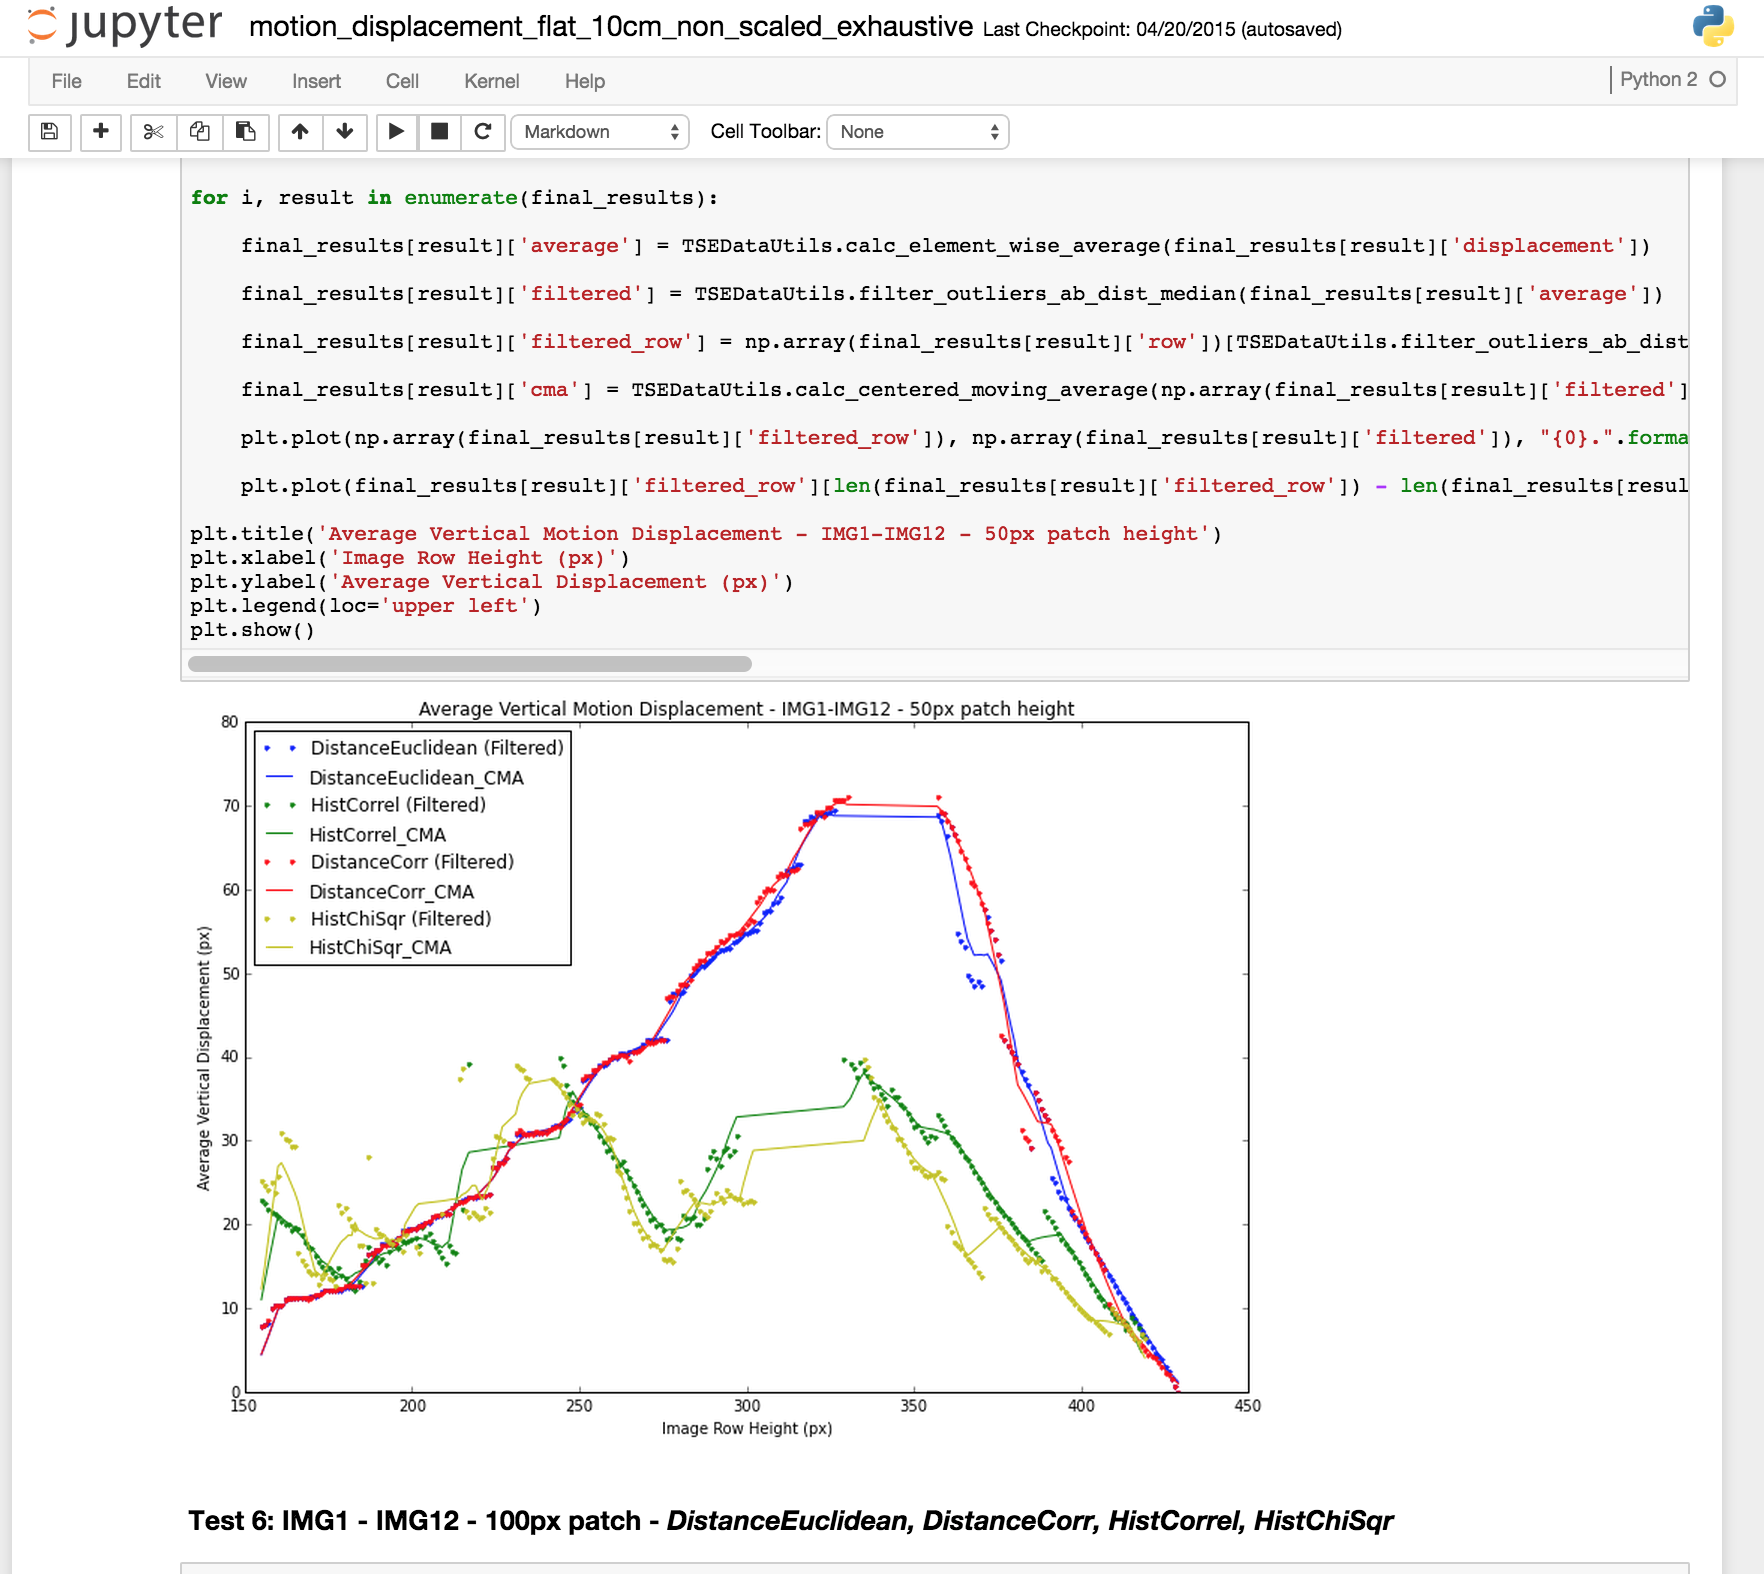
\includegraphics[width=0.55\textwidth]{images/ipython.png}
  \end{center}
  \vspace{-10pt}
  \caption{Example screenshot of the iPython web-based interface running the Python testing rig and displaying the subsequent results all from within a single `notebook'.}
     \label{fig:ipython}
  \vspace{-10pt}
\end{wrapfigure}

A major feature provided within \textit{iPython} is the ability to \textit{interactively} write and run Python code within isolated computational environments known as `notebooks'\footnote{\url{http://ipython.org/notebook.html}}. By communicating with the test rig programmatically, it was possible to define all of the required test parameters within Python code, before passing these over to the test rig in order to then start the tests. Should any changes need to be made, this was accomplished within the web-based user interface, without the need for any interaction with the command line whatsoever. By creating multiple notebooks for each experiment, it was even possible to instruct iPython to automatically trigger either a selection, or indeed all of the tests for each experiment to start at the same time. 


Through the use of the \textit{Matplotlib} library \cite{matplotlib}, the results for each experiment were plotted automatically upon the completion of the test rig before being embedded into the same `notebook' that contained the Python code used to define and initiate that very same test. This meant in effect, that it had become possible to analyse all of the input and output of a single test, performed as part of specific experiment, all within one ``document" (Figure \ref{fig:ipython}).

\subsection{Software Testing}

For testing aspects of the software (predominantly the testing rig and implementations of template matching methods), standard software-based testing practices were adopted. This constituted mainly of unit tests written to test for each specific function written in code, and regression tests for confirming that software continued to work as expected following the correction of a bug.

For unit tests written in Python, the \textit{Nose}\footnote{\url{https://nose.readthedocs.org/en/latest/}} third-party testing framework was selected in favour of the default testing framework (\textit{unittest}), due to its ability to generate code coverage reports in partnership with the \textit{Coverage.py}\footnote{\url{http://nedbatchelder.com/code/coverage/}} library. This was later enhanced by integrating with the \textit{Coveralls.io}\footnote{\url{https://coveralls.io/r/cgddrd/CS39440-major-project}} web service (Figure \ref{fig:coveralls}), which provided automatic analysis and notification of changes in the level of code coverage following each new commit to the remote project git repository hosted at Github.

\begin{figure}[ht!]
\centering
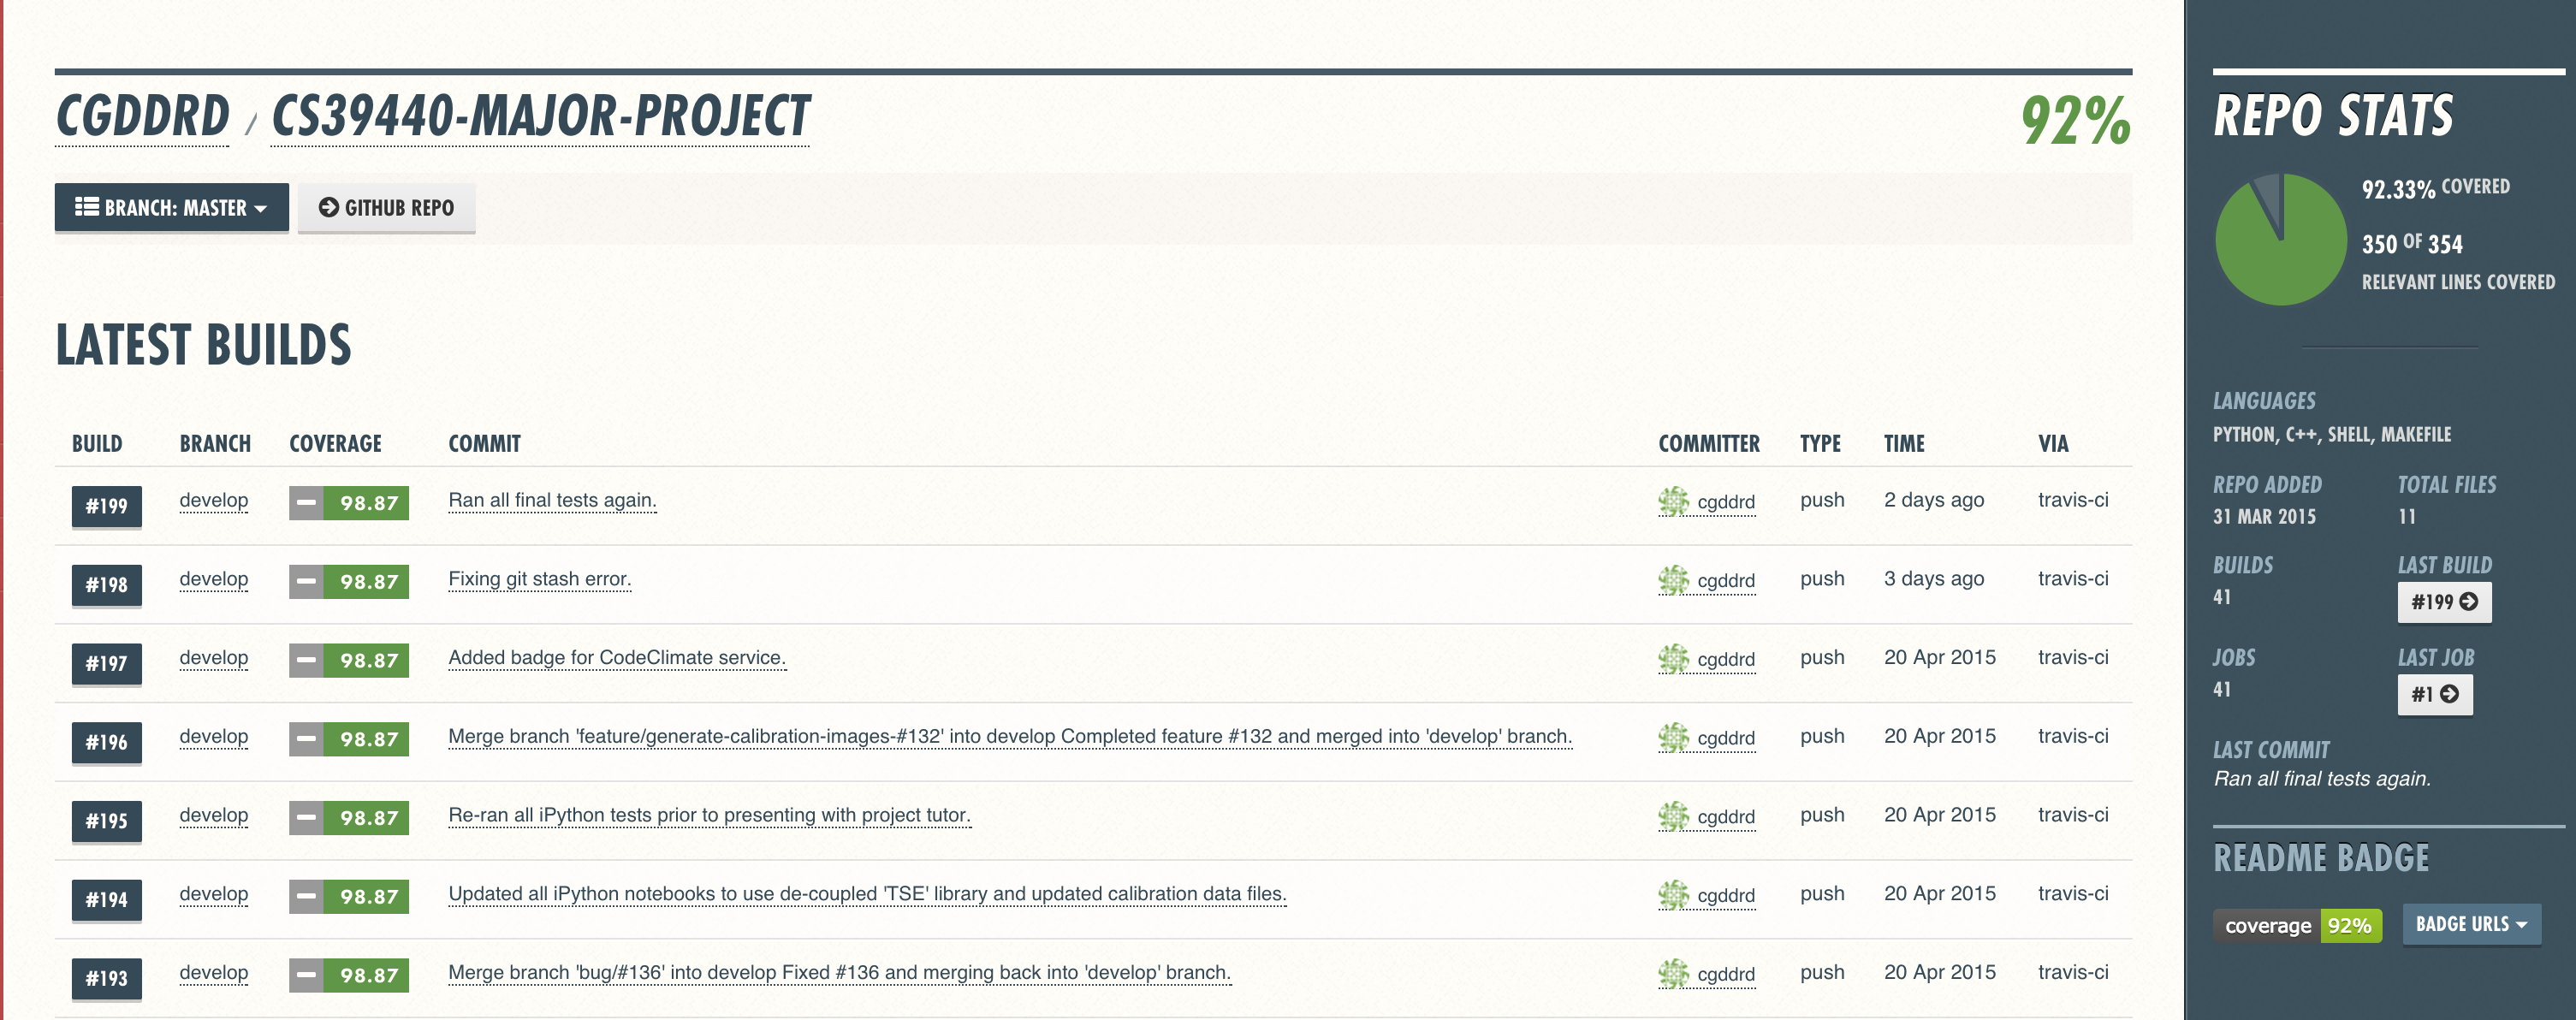
\includegraphics[scale=0.28]{images/coveralls.png}
  \caption{Example screenshot of the Coveralls.io\footnote{\url{https://coveralls.io/r/cgddrd/CS39440-major-project}} web interface providing a breakdown of unit test code coverage.}
     \label{fig:coveralls}
\end{figure} 

\section{Experiment Methods}

This section provides an overview the three main experiment methods conducted within the scope of the project investigation, that all relate to the first primary research aim discussed in Section \ref{primary-aims}.

While not specifically intended, as the investigation progressed the focus began to change from  exploring a series of reasonably ``generalised" research aims, to instead concentrating almost exclusively on one small, but very important aspect; \textit{ensuring that accurate results for appearance-based motion displacement could continue to be achieved, across terrain lacking any significant features and/or demonstrating highly repetitive patterns}.

  As a result, each of the three primary experiments detailed in this section, focussed on testing and evaluating subsequent evolutions of the same fundamental approach, with the hope of eventually identifying a method that could provide sufficient accuracy across all types of potential terrain. 
 
\subsection{Experiment 1: Template Matching (Multiple Small Patches)}
\label{ex1}

This experiment focussed on the extraction and subsequent matching of multiple overlapping square patches in order to provide an appearance-based approach to performing dense optical flow, in the hope that it would be possible to generate a vertical displacement model confirming the predicted behaviour stated in Section \ref{hypo-model}. 

The method followed a \textit{six-stage} process (Figure \ref{fig:ex1process})to build the vertical displacement model used later to compare vertical motion displacement for the identification of obstacles and terrain slopes:

\begin{enumerate}
\item Import two consecutive images from one of the test datasets, convert both images from RGB to HSV colour space, subsequently ``remove" the 'V' channel by setting all the corresponding channel values to 0.
\item Extract a percentage-width region of interest (ROI) from centre of first image (discussed further in Section \ref{hypo-calib}).
\item Extract square patches of a fixed size around the centre each pixel within the extracted ROI. These patches would act as the \textit{templates} when performing the appearance-based template matching. 
\item For each patch extracted from image one, move down through a localised search window (column) in image two searching for the best match against the template patch.
\item Identify the patch within the localised search window that provides the ``best match" via appearance-based matching.
\item Average all measured vertical displacement values for each pixel along a given row, removing outliers by ignoring any displacements that lie outside of (2 x standard deviation) of the mean, before appending to the vertical displacement model.
\end{enumerate}

\clearpage
\begin{figure}[ht!]
\centering
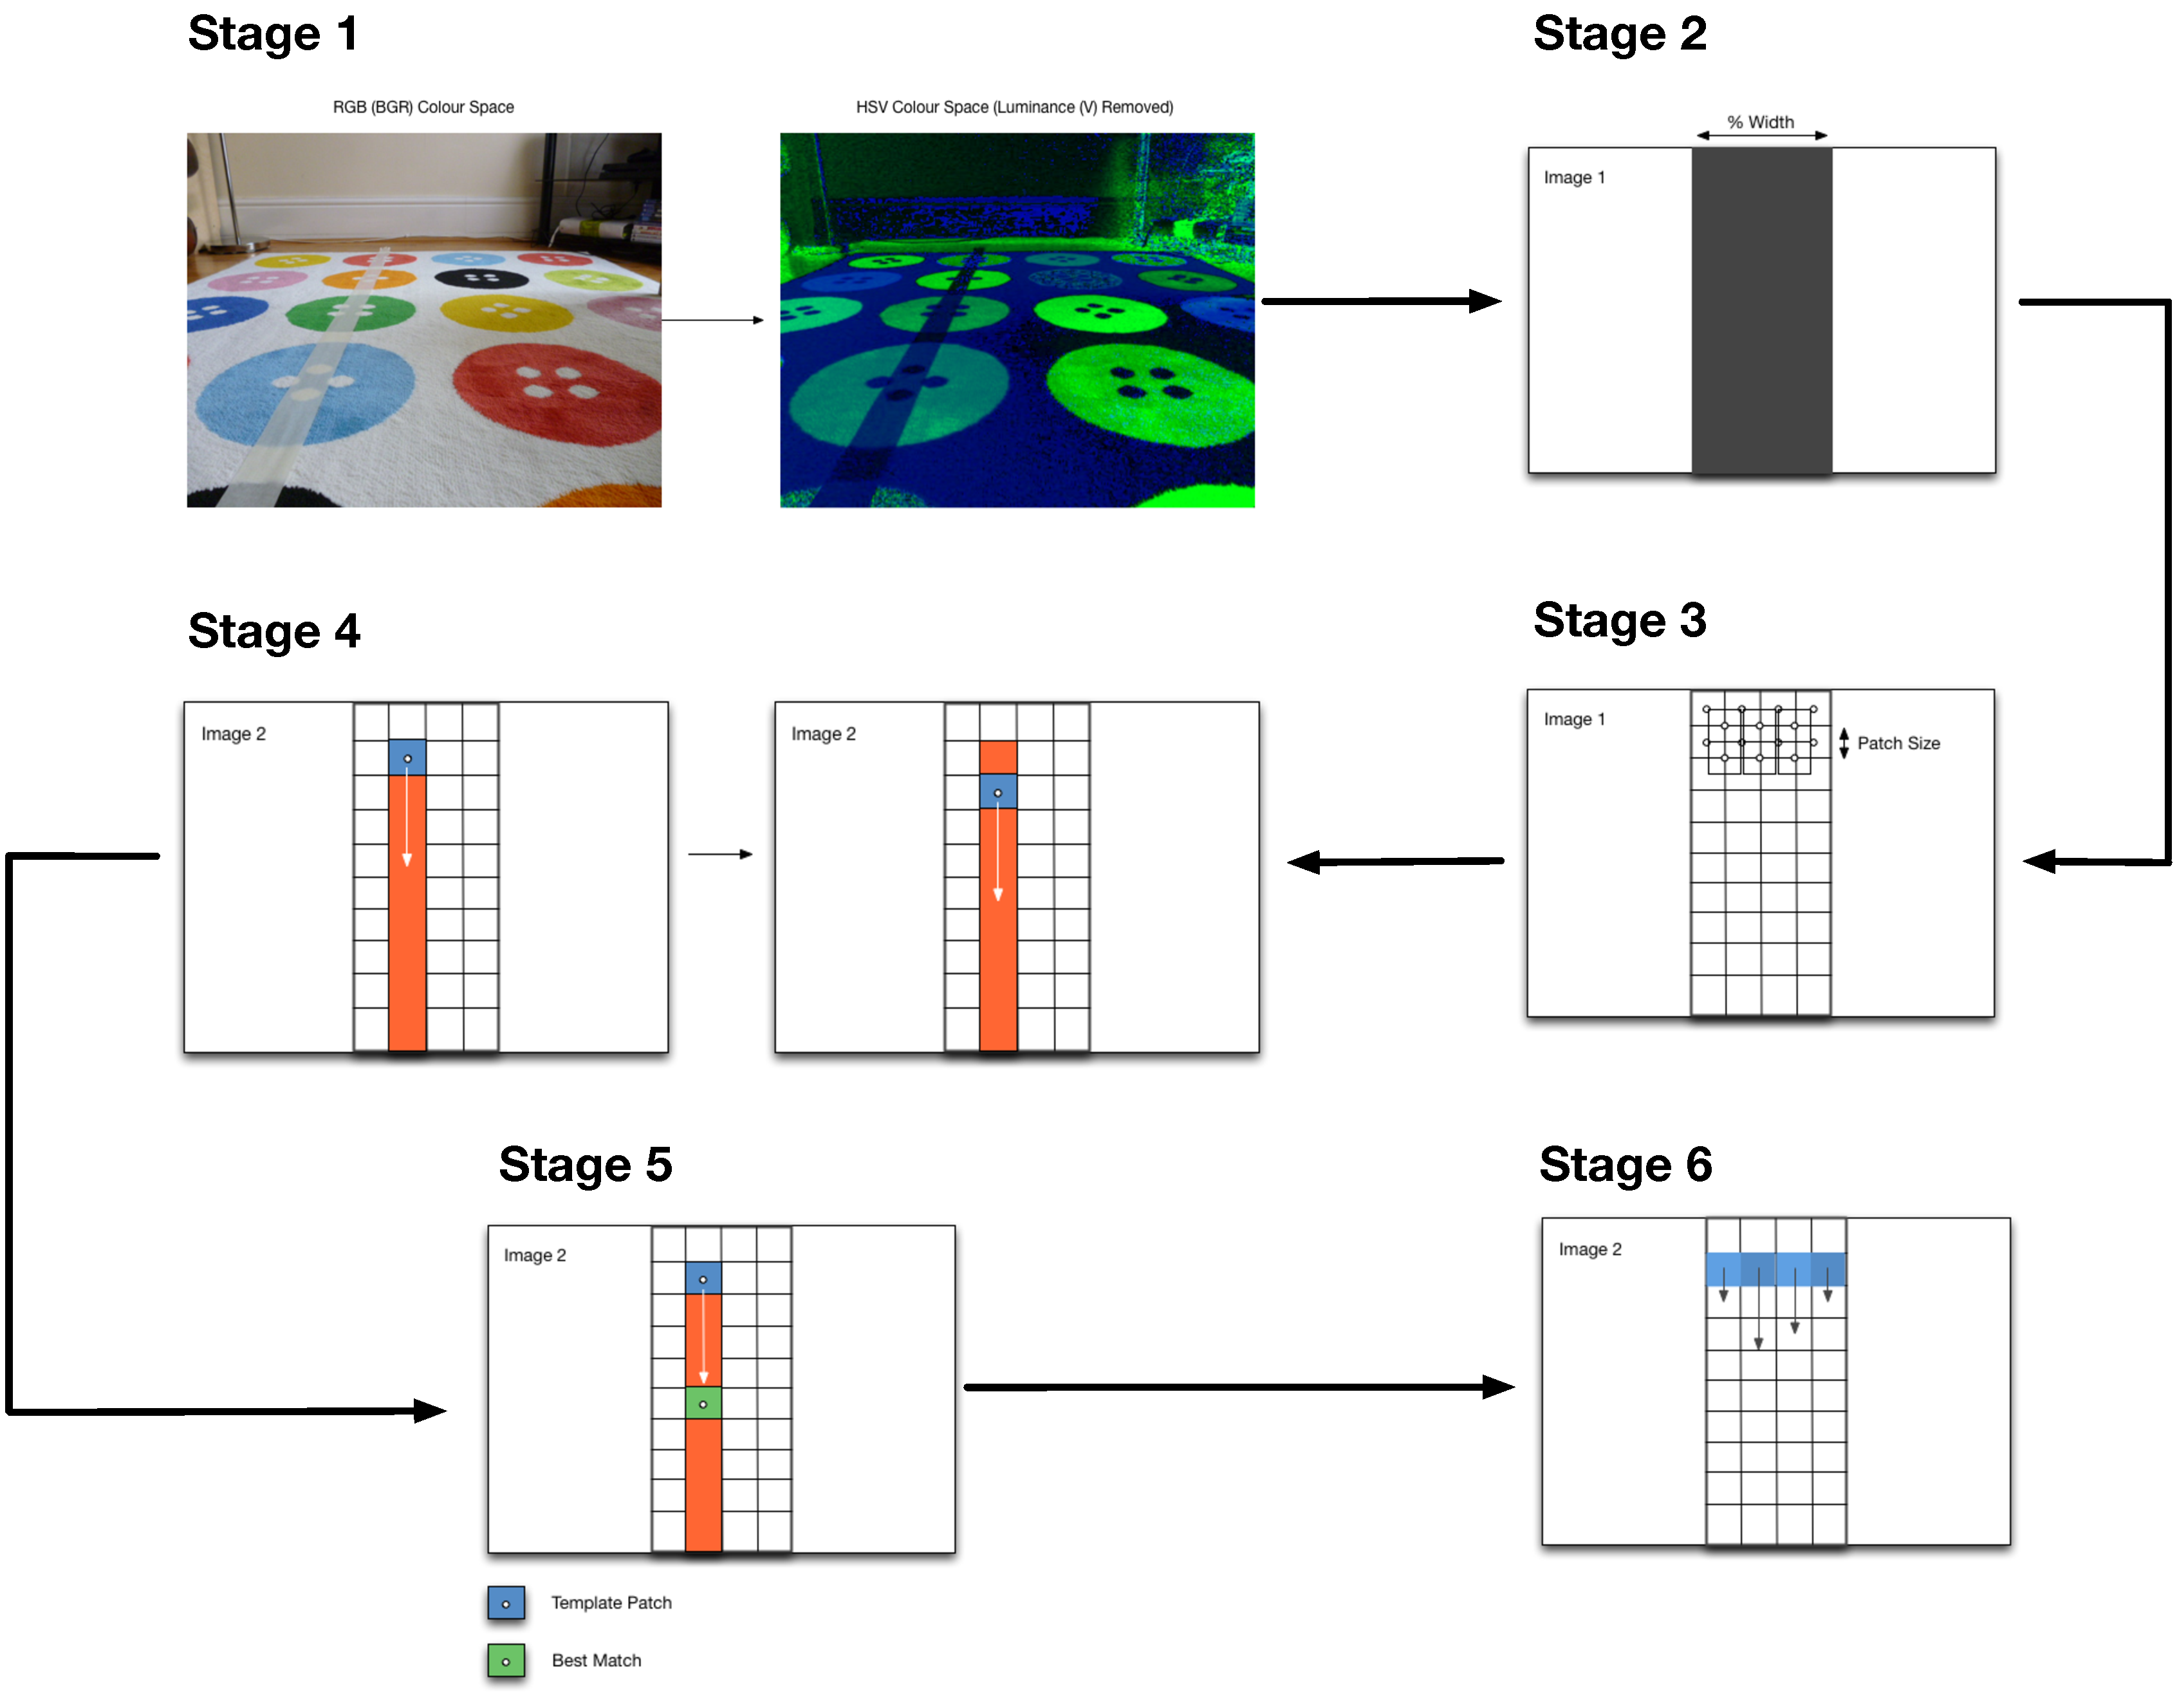
\includegraphics[scale=0.25]{images/ex1stages.pdf}
  \caption{Process model for the method undertaken within Experiment 1 to evaluate the use of multiple small-sizes template patches in order to infer the vertical displacement of corresponding features between two consecutive images.}
\label{fig:ex1process}
\end{figure} 

\clearpage
\subsection{Experiment 2: Template Matching (Full-width Patches - Non-Scaled)}

This second experiment focussed on establishing if adopting \textit{larger patches} in fewer numbers provided better appearance-based matching accuracy than the method attempted in the first experiment of using many more, but critically \textit{much smaller} overlapping patches 

 While the underlying method remained the same as in the first experiment, some crucial changes had been made:
 
 \begin{itemize}
 	\item Extracting a central region of interest relative to the \textit{ground plane}, as opposed to extracting a fixed-width column from the image plane.
 	\item Moving away from multiple overlapping small patches, in favour of adopting a single, \textit{full-width} patch to represent a single row in the image. 
 \end{itemize}

\subsubsection{Exhaustive \& Non-Exhaustive Searching}
\label{searching}

As part of the localised search detailed in stage five of the method from experiment one (Section \ref{ex1}), the current implementation saw the adoption of \textit{non-exhaustive} searching behaviour for identifying the corresponding region within a localised search window that provided the ``best match" overall. 

The motivation behind non-exhaustive searching prevented the need to continue searching down the entire localised search window column, if it was believed that the best match for that search window had \textit{already been located}. 

\begin{wrapfigure}{r}{0.6\textwidth}
\vspace{-20pt}
  \begin{center}
    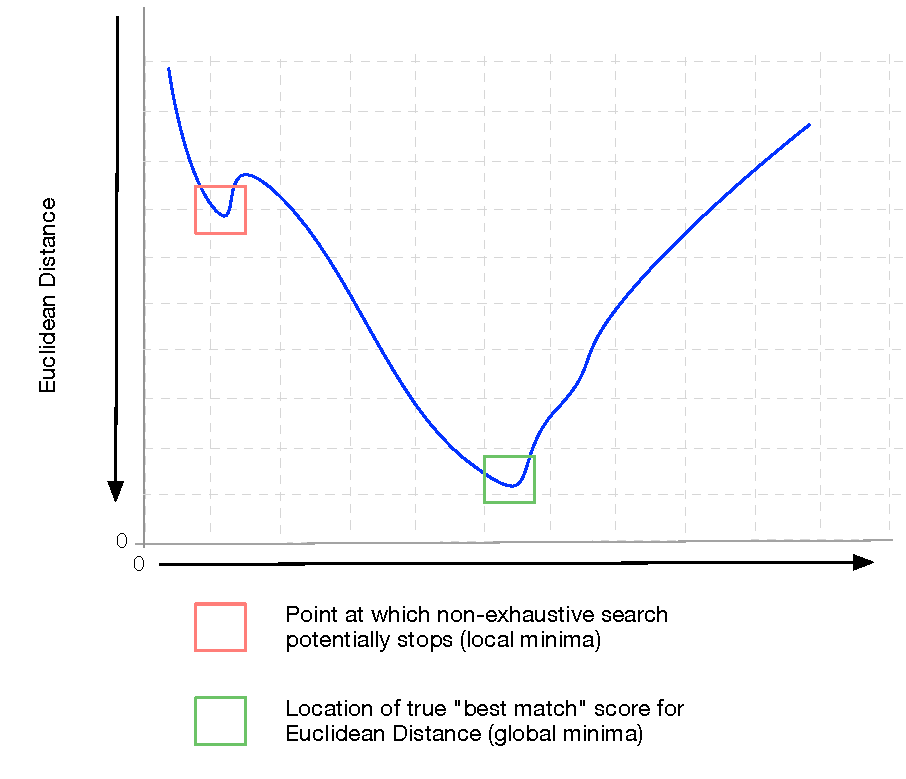
\includegraphics[width=0.55\textwidth]{images/ed.pdf}
  \end{center}
  \vspace{-10pt}
  \caption{Example of potential early termination of non-exhaustive search due to entering local minima caused by noise, rather than global minima which represents to true best match.}
     \label{fig:ed}
  \vspace{-10pt}
\end{wrapfigure}

The criteria for stopping a search, focussed around the observed scoring behaviour of appearance-based matching metrics, where in the case of Euclidean Distance, the score would demonstrate a uniform decline, until reaching a minima representing the best possible match, before subsequently beginning to rise once more (Figure \ref{fig:ed}). That is to say, the search should continue until such a time as the score no longer continues to become progressively ``better", at which point the last score recorded \textit{previously} to this would also represent the best possible score for that search (See Appendix B - Algorithm \ref{appen:code2} for an pseudocode outline for this approach).

While in theory this approach appeared reasonable, it was later identified that it had the potential to suffer greatly upon the onset of image noise. The issue that was presented, involved the search terminating prematurely as a result of arriving at a local minima caused by noise, rather than terminating at the ``global" minima that represented the \textit{true} best match within the search window column (Figure \ref{fig:ed}). 

In order to confirm this observation, all of the tests conducted over experiments two and three were run twice, one time using the non-exhaustive search, and the other using an exhaustive search.

\subsubsection{Perspective Distortion Calibration Tool}

A consequence of choosing to isolate a central region-of-interest relative to the ground plane rather than the image plane, described how the shape of the search region would become subject to distortion caused by changes in perspective, where the ground within the image appears to `converge' towards a central point along the horizon line.

As template patches were now expected to span the \textit{full width} of the region of interest, it became necessary for the width of the extracted template patches to increase as the search moved towards the bottom of the image. 

In order to achieve this, the system required knowledge of what the \textit{corresponding width} should be for every \textit{image row} that represented the ground plane (i.e from the central horizon line to the bottom of the image). 

\begin{wrapfigure}{r}{0.6\textwidth}
\vspace{-20pt}
  \begin{center}
    
\includegraphics[width=0.55\textwidth]{images/calib.jpg}
  \end{center}
  \vspace{-10pt}
  \caption{Example output from perspective calibration utility tool highlighting the identified region of interest along the ground plane for dataset one.}
     \label{fig:calib}
  \vspace{-10pt}
\end{wrapfigure}

To provide this information, a small utility tool was developed that would allow a user to export a calibration data file defining the shape of required region of interest positioned along the ground plane (Figure \ref{fig:calib}). 

The Python application employed the mouse and keyboard listener features included within the \textit{Matplotlib} library \cite{matplotlib} to create a minimal graphical user interface that enabled the user to define either one or both of the long-side edges that would form the trapezoidal region of interest along the ground plane of the scene within the image. This was achieved through the use of a special `calibration' image from the current image dataset containing a guide (i.e. tape along the floor) that would provide a visual indication as to the effects of the observed perspective distortion. 

Following the selection of line end-points via mouse clicks, the application made use of the \textit{Bresenham line algorithm} \cite{bresenham} to linearly interpolate the remaining coordinate points in order to arrive at what would become the full long-side edge of the region of interest. 

For convenience, the application also included a feature whereby the user could horizontally \textit{reflect} an edge defined on one side of the image over to the other. This helped to ensure that the area in which the region of interest occupied remained \textit{horizontally symmetrical}.

Upon the definition of both long-side edges forming the trapezium-shaped area along the ground plane, the application would finally export calibration data, by calculating the distance in pixels between the two corresponding `X' coordinates that positioned along both of the opposite edges with respect to each row.

\subsection{Experiment 3: Template Matching (Full-width Patches - Geometric Scaling)}
\label{tm-scaled}

The final experiment aimed to investigate if it could be possible to further increase the matching accuracy reported in experiment two, by adding the additional step of \textit{geometrically scaling} the current template patch as the search progressed down the trapezoidal-shaped region of interest.

\begin{wrapfigure}{l}{0.5\textwidth}
  \begin{center}
    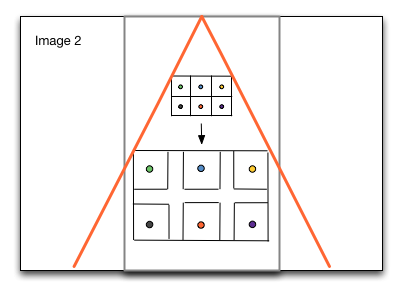
\includegraphics[width=0.45\textwidth]{images/scaling.png}
  \end{center}
  \vspace{-10pt}
  \caption{Diagram depicting process of geometrically scaling the 2D position coordinates of the pixels from the template patch, in order to subsequently match with the pixels located in the corresponding position within the previously-scaled search window.}
  \label{fig:scaled}
  \vspace{-10pt}
\end{wrapfigure}

The underlying theory adopted for this proposal related back to the idea that, if a camera was to move \textit{closer} to an object on the ground between the capture of two consecutive images, then upon the subsequent visual inspection of both these images, it would be possible to observe that the same object appears \textit{larger} within the second image than in the first. Thus, by geometrically \textit{scaling} the template patch (extracted from the first image), it may then be possible to find a better match within the second image, as a result of the partial scene represented by the template patch subsequently appearing to have become visually larger within the second image due to the effects of perspective distortion (Figure \ref{fig:scaled}).

In the context of this experiment, the specific task of geometrically-scaling and subsequently matching the template patch took form of the following stages:

\begin{enumerate}
	\item Obtain the width and height of the current template patch;
	\item Obtain the calibrated \textit{width} of the search window with respect to the current image row;
	\item Calculate the independent scale factor for the width and height between the template patch and the search window where:
	
	\begin{equation}
		\text{Scale Factor} = \frac{\text{Target Value}}{\text{Current Value}}
	\end{equation}
	 
	\item Treating each pixel as a 2D coordinate in geometric space, scale the position of each pixel coordinate within the template patch relative to the position of centre coordinate:

	\begin{gather} 
 \vec{CP} = (P_{x} - C_{x}, P_{y} - C_{y})
 \\
\vec{CPS} = \begin{bmatrix} \vec{CP}_{1} \\ \vec{CP}_{2} \end{bmatrix}\begin{bmatrix} S_{Width} & 0 \\ 0 & S_{Height} \end{bmatrix} = \begin{bmatrix} \vec{CP}_{1}S \\ \vec{CP}_{2}S \end{bmatrix}
\\
P_{ScaleTarget} = (C_{x} + \vec{CPS}_{1}, C_{y} + \vec{CPS}_{2}) 
\end{gather} 
		
where $C$ refers to the centre position coordinate within the template patch, $P$ refers to the original pixel coordinate position, $S_{Width}$ and $S_{Height}$ refer to the scale factor for the width and height respectively, and $P_{ScaleTarget}$ refers to the final scaled position of $P$. 

\item For each scaled pixel coordinate, extract the value of the pixel at the \textit{corresponding position} with the search window and add to a temporary ``image" data structure.

\item Perform ``standard" template matching between the original template patch, and the newly created temporary image.
	
\end{enumerate}

Due to the reliance that appearance-based similarity measures hold on the evaluation of \textit{corresponding} pixel values between two images, a key condition of using such an approach is that both of the images to be compared demonstrate an \textit{equal size} (i.e. there are the \textit{same number of pixels in both images}). One of key challenges associated with the proposed method was how to still uphold this condition, while also wanting to potentially compare images of two different sizes (i.e. original template patch and larger search window). 

\begin{figure}[ht!]
\centering
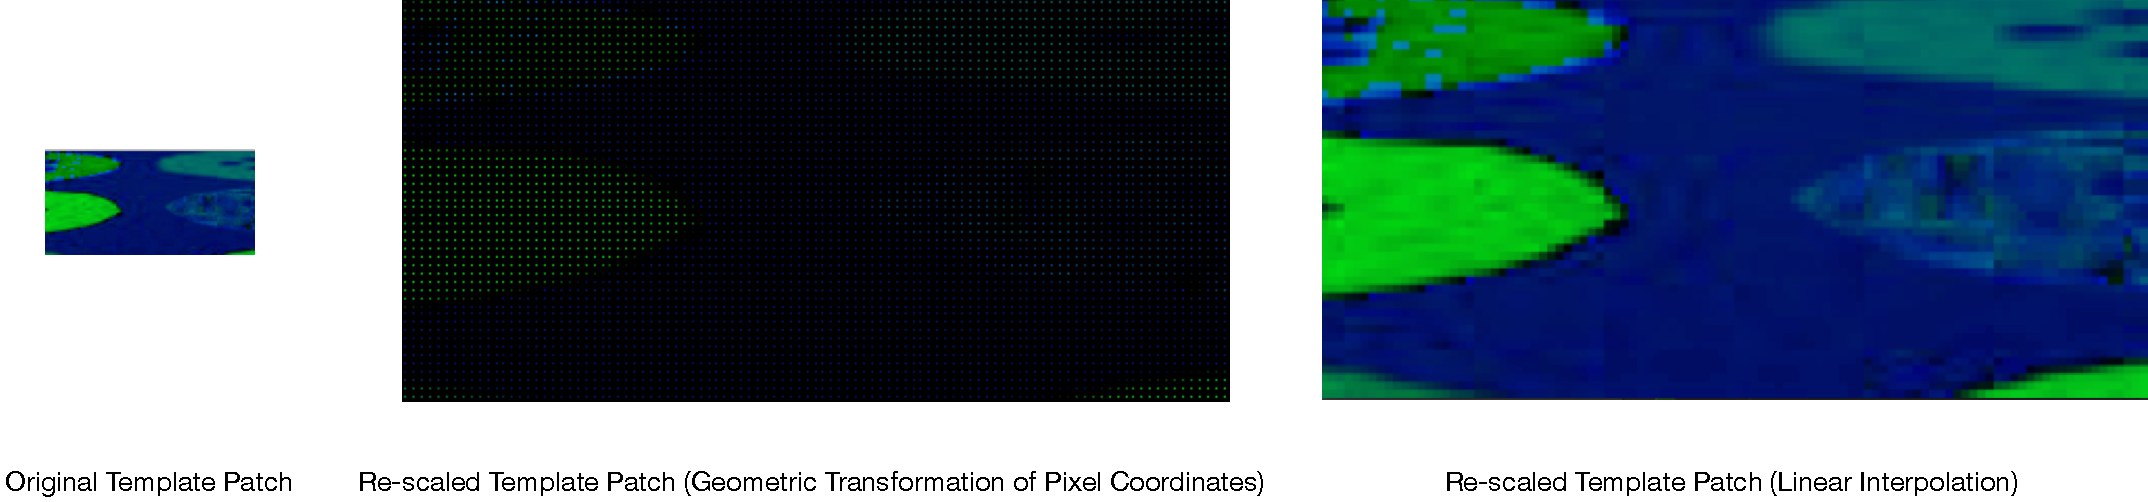
\includegraphics[scale=0.4]{images/scaling_types.pdf}
  \caption{Comparison between the various approaches of performing scaling of the original template patch image. In the case linear interpolation, additional information has been added to image as a result of ``estimating" the colour that lies between two original pixels. }
\label{fig:scaletypes}
\end{figure} 

The solution to this issue lay in the \textit{extraction} of pixels from the larger search window, whose 2D position corresponded to the \textit{scaled} position of each pixel in the original template patch. By subsequently comparing the original template patch, with the collection of newly-extracted corresponding pixels from the search window, it was possible to continue to use all of the appearance-based similarity measures as had previously been utilised in experiments one and two. 

Another important realisation, was that no additional information regarding the scene represented by the two images was being either \textit{lost} or \textit{gained} as a result of utilising pixel 2D position scaling and subsequent extraction. This however, would not have been the case had the method naively attempted to ``resize" the template patch in order to have the same dimensions as the larger search window (Figure \ref{fig:scaletypes}). 

This is because to enlarge the entire template patch image, it would be necessary to linearly interpolate between each of the original pixels, causing new, and most likely incorrect information to be added prior to perform appearance-based matching, which subsequently may have caused the results to be very different to the actual true similarity between the current template patch and search window.

\subsubsection{Verification of Geometric Scaling Approach}

In order to test that the implemented approach to geometrically scaling template patch pixels could was working as expected, a simple test was devised making use of an artificially generated test image (Figure \ref{fig:graphpic}) to confirm that the approach could successfully match two identical objects within an image, whereby the only theoretical difference between them was a scale transformation.

\begin{figure}[ht!]
\centering
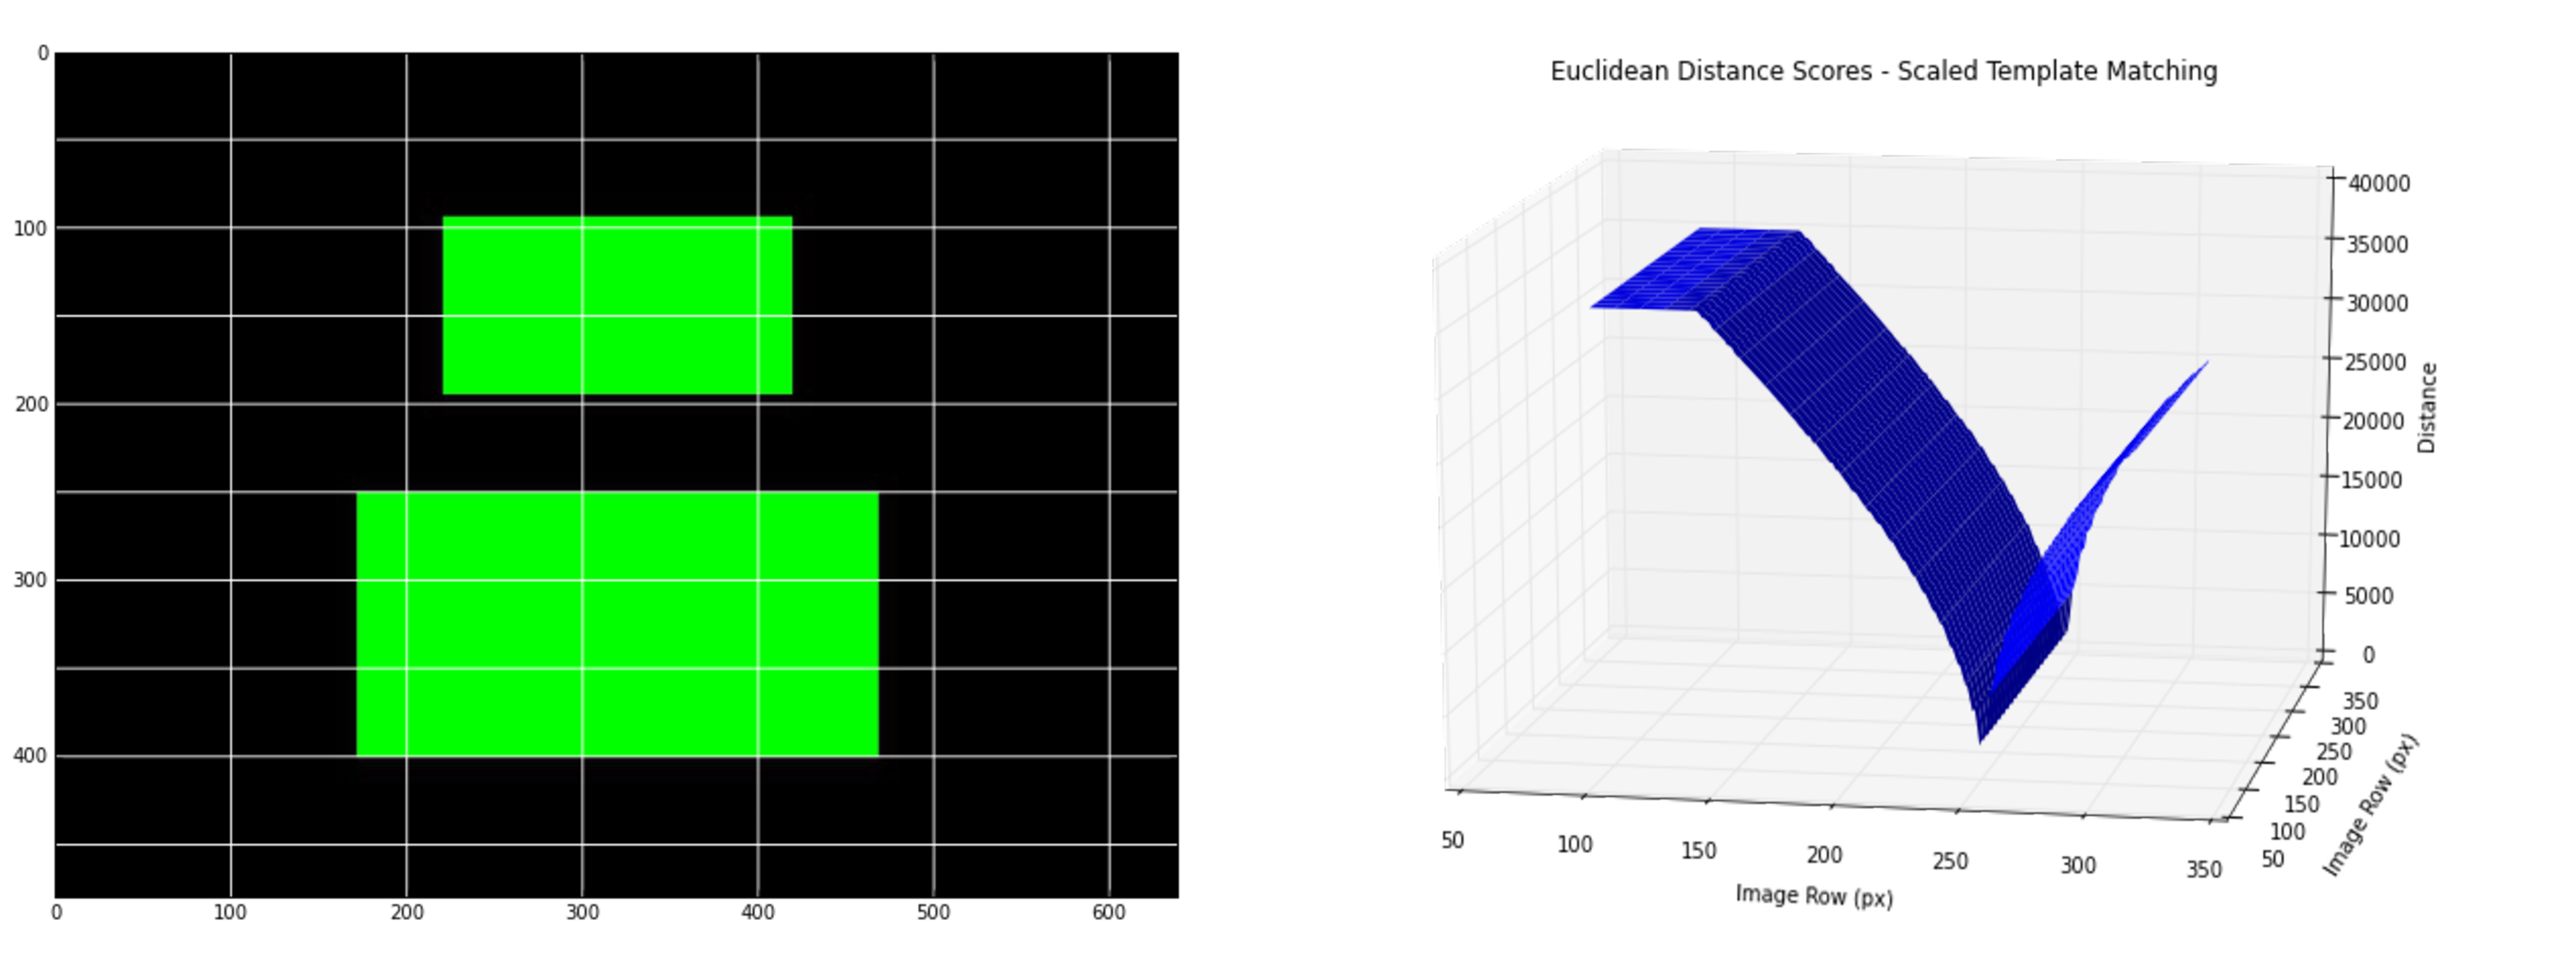
\includegraphics[scale=0.3]{images/3d_graph.pdf}
  \caption{Results of the verification test for the approach towards geometric scaling of template patch pixel coordinates. On the left is the calibrated test image (grid applied only for result analysis) where the two rectangles are identical apart from a single scaling transformation. On the right is the plotted Euclidean Distance scores for the geometric search.}
\label{fig:graphpic}
\end{figure} 

The results of this test (Figure \ref{fig:graphpic}) indicated that the approach was working successfully, given by the clear improvement (i.e. sharp decline) in the Euclidean Distance score as soon as the scaled template patch search arrives at the top of the scaled template patch (Row 250) whereby there is a complete alignment between the scaled version of the top green rectangle, and the bottom rectangle. As the search continues, this alignment moves and the score becomes progressively worse.
